\section{مقدمه}
\label{sectio:design:preface}
در این فصل از پژوهش روش طراحی منطق دامنه بر اساس تبادل ناهمگام پیغام ارائه شده است. تلاش شده است تا تطابق طراحی با مدل بازیگر در حد امکان حفظ شود. با توجه به تمرکز این بخش بر روش طراحی منطق دامنه و به هدف ایجاد شفافیت و افزایش قابلیت فهم نکات و الگوهای مطرح شده در روش، تصمیم به استفاده از یک سیستم نمونه به عنوان مثال گرفته شد. کلیه‌ی نکات مطرح شده در ادامه‌ی این بخش در قالب این مثال ارائه خواهند شد. در انتخاب سیستم نمونه نکات ذیل مورد توجه قرار گرفته‌ است:
\begin{enumerate}
\item \textbf{دامنه‌ی سیستم انتخابی:}
رده‌ی دامنه‌ی سیستم انتخاب شده به طور کلی سیستم‌های اطلاعاتی\LTRfootnote{Information System} است. اولین دلیل انتخاب این رده این است که در این نوع دامنه همروندی به طور ذاتی وجود ندارد و به همین دلیل زمینه‌ی مقایسه‌ی طراحی بر اساس تبادل ناهمگام با  طراحی‌های شیءگرای ترتیبی فراهم می‌شود. با توجه به اینکه یکی از موارد مقایسه‌ی این نوع طراحی با طراحی شیءگرای ترتیبی تفاوت کارایی این دو رویکرد است، دامنه‌ی انتخاب شده باید در حالت ترتیبی هم قابلیت اضافه شدن همروندی را داشته باشد. سیستم‌های اطلاعاتی از این حیث نیز انتخاب مناسبی محسوب می‌شوند چرا که در اکثر پیاده‌سازی‌های عملیاتی، علیرغم داشتن طراحی ترتیبی، به وسیله‌ی ریسمان‌هایی که وب‌سرورها برای پاسخگویی به درخواست‌های همزمان کاربران ایجاد می‌کنند، دارای خاصیت همروندی نیز می‌گردند. به همین دلیل در بخش ارزیابی می‌توانیم با شبیه‌سازی عملیات وب‌سرورها، کارایی و نیز تغییرپذیری دو نوع طراحی مذکور را ارزیابی و مقایسه کنیم.
 دلیل دیگر این انتخاب بالا بودن میزان آشنایی جامعه‌ی طراحی شیءگرا با این نوع سیستم‌ها و استفاده‌ی گسترده از این نوع سیستم‌ها می‌باشد. شایان ذکر است که سعی شده است در ارائه‌ی الگوها و نکات استخراج شده از این طراحی بر دامنه‌ی انتخاب شده تکیه‌ نشود. دامنه‌ی سیستم نمونه نیز یک سیستم آموزشی انتخاب شده است. با توجه به اینکه استفاده کنندگان این پژوهش جامعه‌ی دانشگاهی هستند، آشنایی این جامعه با سیستم آموزشی دلیل اصلی انتخاب آن بوده است. 
\item \textbf{ بزرگی منطق دامنه:}
از نظر میزان بزرگی سیستم (تعداد کلاس‌ها و موارد کاربرد\LTRfootnote{use cases})،‌  سعی شده منطق حداقل بزرگی و پیچیدگی را داشته باشد تا ضمن امکان مشاهده‌ی الگوهای مختلف، نیازی به تکرار نکات طراحی برای مولفه‌های متعدد و مشابه نباشد. 
\end{enumerate} 

\section{معرفی یک سیستم آموزش ساده }
\label{section:eduIntro}
همان‌طور که در بخش \ref{sectio:design:preface} ذکر شد،‌ یک سیستم آموزش کوچک به عنوان مدل طراحی انتخاب شده است. در ادامه‌ی این بخش ابتدا موارد کاربرد\LTRfootnote{use cases} انتخاب شده در این سیستم را توصیف می‌کنیم و سپس با توجه به‌ آنها مدل دامنه\LTRfootnote{Domain Model} سیستم را در قالب نمودار کلاس بیان می‌کنیم.

\subsection{موارد کاربرد}
در این بخش موارد کاربرد انتخاب شده برای سیستم آموزش معرفی می‌شوند. لازم به تأکید است که علیرغم این که این موارد کاربرد، مرتبط و هماهنگ با موارد کاربرد یک سیستم آموزش واقعی هستند، به هیچ عنوان تمام موارد کاربرد مورد نیاز برای ساختن سیستم واقعی را شامل نمی‌شوند و علاوه‌ بر آن، موارد انتخاب شده دارای جزئیات و دقت کافی برای پوشش فرایند‌های واقعی نیستند. در ادامه‌ی این بخش، هر \gls{مورد کاربرد} در قالب یک جدول توصیفی ارائه شده‌ است.


%%%%%%%%%%%%%%%%%%%%%%%%%%%%%
%%%%  GPA
%%%%%%%%%%%%%%%%%%%%%%%%%%%%%
\begin{table}
\begin{center}
\begin{tabular}{|p{5cm}|p{10cm}|}
	\hline
	\textbf{نام مورد کاربرد} &
درخواست محاسبه‌ی معدل ترم دانشجو\\
	\hline
	\textbf{بازیگر(ان)} &
کاربر\\
	\hline
	\textbf{شروع می‌شود زمانی که} &
درخواست محاسبه‌ی معدل ترم وارد سیستم می‌شود.\\
	\hline
	\textbf{پیش‌شرط‌ها} &
دانشجو و ترم در سیستم تعریف شده باشند.\\
	\hline
	\textbf{جریان اصلی} &
۱. درخواست محاسبه‌ی معدل دانشجو در ترم مربوطه وارد سیستم می‌شود.\newline
۲. سیستم سوابق تحصیلی دانشجو در ترم مربوطه را بررسی ‌می‌کند. معدل ترم با توجه به نمرات اخذ شده و تعداد واحد هر درس محاسبه و اعلام می‌شود. در صورتی که نمره‌ی درس سابقه‌ای وارد نشده باشد، درس مربوطه در محاسبه‌ی معدل لحاظ نمی‌گردد.\\
	\hline
\textbf{جریان استثنا ۱} &
۲.الف) در صورتی که دانشجو هیچ واحدی در ترم جاری اخذ نکرده باشد پیغام خطای مناسب صادر می‌شود و جریان اصلی خاتمه می‌یابد.\\
	\hline
%	\textbf{جریان استثنا ۲} &
%۴-ج. رمز وارد شده نامعتبر است، پیام خطای رمز نامعتبر است به کاربر نمایش داده شده و تراکنش متوقف می‌شود\\
%	\hline
	\textbf{تمام می‌شود زمانی که} &
معدل دانشجو اعلام می‌شود یا خطای مناسب صادر می‌گردد.\\
	\hline
%	\textbf{پس شرط‌ها} &
%کاربر موجودی کارت و یا خطای تراکنش را مشاهده کرده است.\\
%	\hline
\end{tabular}
\caption{\label{table:uc_gpa} توصیف مورد کاربرد محاسبه‌ی معدل یک دانشجو در یک ترم}
\end{center}
\end{table}

%%%%%%%%%%%%%%%%%%%%%%%%%%%%%
%%%%  Take Course
%%%%%%%%%%%%%%%%%%%%%%%%%%%%%
\begin{table}
\begin{center}
\begin{tabular}{|p{4cm}|p{12cm}|}
	\hline
	\textbf{نام مورد کاربرد} &
درخواست اخذ یک ارائه در یک ترم\\
	\hline
	\textbf{بازیگر(ان)} &
کاربر\\
	\hline
	\textbf{شروع می‌شود زمانی که} &
درخواست اخذ ارائه وارد سیستم می‌شود.\\
	\hline
	\textbf{پیش‌شرط‌ها} &
۱. ‌انتخاب واحد در ترم امکانپذیر باشد. (رجوع کنید به جداول \ref{table:uc_enableofferings}و\ref{table:uc_disableofferings})\\
	\hline
	\textbf{جریان اصلی} &
۱. سیستم کنترل می‌کند که دانشجو در ترم‌های قبل این درس را نگذرانده باشد.\newline
۲. سیستم کنترل می‌کند که دانشجو در ترم‌ جاری این درس را اخذ نکرده باشد.\newline
۳. سیستم کنترل می‌کند که دانشجو تمام پیش‌نیاز‌های این درس را با موفقیت گذرانده باشد.\newline
۴. سیستم کنترل می‌کند که تعداد واحد‌های اخذ شده توسط دانشجو در این ترم پس از اخذ این درس بیشتر از ۲۰ نشود.\newline
۵. سیستم یک سابقه از ارائه‌ی انتخاب شده برای دانشجو تشکیل می‌دهد و آن را در سوابق دانشجو ثبت می‌کند.\\
	\hline
\textbf{جریان استثنا ۱} &
۱.الف)در صورتی که دانشجو قبلا این درس را گذرانده باشد، خطای ''درس انتخاب شده قبلاً گذرانده شده است`` صادر می‌شود و جریان اصلی خاتمه می‌یابد.\\
	\hline
\textbf{جریان استثنا ۲} &
۲.الف)در صورتی که دانشجو در ترم جاری این درس را اخذ کرده باشد، خطای ''این درس در ترم جاری قبلاً اخذ شده است`` صادر می‌شود و جریان اصلی خاتمه می‌یابد.\\
	\hline
\textbf{جریان استثنا ۳} &
۳.الف)در صورتی که دانشجو یکی از پیش‌نیاز‌های درس‌ را نگذرانده باشد، خطای ''انتخاب بیشتر از ۲۰ واحد در ترم مجاز نمی‌باشد`` صادر می‌شود و جریان اصلی خاتمه می‌یابد.\\
	\hline
\textbf{جریان استثنا ۴} &
۴.الف)در صورتی که تعداد واحد‌های اخذ شده توسط دانشجو در این ترم پس از اخذ این درس بیشتر از ۲۰ شود، خطای ''انتخاب بیشتر از ۲۰ واحد در ترم مجاز نمی‌باشد`` صادر می‌شود و جریان اصلی خاتمه می‌یابد.\\
	\hline
	\textbf{تمام می‌شود زمانی که} &
سابقه‌ی جدید در سوابق دانشجو ثبت می‌شود و یا خطای مناسب صادر می‌گردد.\\
	\hline
\end{tabular}
\caption{\label{table:uc_takecoure} توصیف مورد کاربرد اخذ یک ارائه توسط یک دانشجو در یک ترم}
\end{center}
\end{table}

%%%%%%%%%%%%%%%%%%%%%%%%%%%%%
%%%%  DISABLE_TERM_OFFERINGS
%%%%%%%%%%%%%%%%%%%%%%%%%%%%%
\begin{table}
\begin{center}
\begin{tabular}{|p{5cm}|p{10cm}|}
	\hline
	\textbf{نام مورد کاربرد} &
درخواست غیر فعال کردن ارائه‌های یک ترم برای انتخاب واحد\\
	\hline
	\textbf{بازیگر(ان)} &
کاربر(مدیر سیستم)\\
	\hline
	\textbf{شروع می‌شود زمانی که} &
درخواست غیرفعال کردن ارائه‌های یک ترم وارد سیستم می‌شود.\\
	\hline
	\textbf{پیش‌شرط‌ها} &
 ترم در سیستم تعریف شده باشند.\\
	\hline
	\textbf{جریان اصلی} &
۱. درخواست غیر فعال کردن ارائه‌های یک ترم وارد سیستم می‌شود.\newline
۲.سیستم تمام ارائه‌های یک ترم را غیرفعال می‌کند.\\
	\hline
	\textbf{تمام می‌شود زمانی که} &
تمام ارائه‌های ترم برای انتخاب واحد غیرفعال می‌شوند.\\
	\hline
	\textbf{پس شرط‌ها} &
انتخاب واحد در ترم امکان پذیر نیست.\\
	\hline
\end{tabular}
\caption{\label{table:uc_disableofferings} توصیف مورد کاربرد غیرفعال کردن ارائه‌های یک ترم برای انتخاب واحد}
\end{center}
\end{table}

%%%%%%%%%%%%%%%%%%%%%%%%%%%%%
%%%%  ENABLE_TERM_OFFERINGS
%%%%%%%%%%%%%%%%%%%%%%%%%%%%%
\begin{table}
\begin{center}
\begin{tabular}{|p{5cm}|p{10cm}|}
	\hline
	\textbf{نام مورد کاربرد} &
درخواست فعال کردن ارائه‌های یک ترم برای انتخاب واحد\\
	\hline
	\textbf{بازیگر(ان)} &
کاربر(مدیر سیستم)\\
	\hline
	\textbf{شروع می‌شود زمانی که} &
درخواست فعال کردن ارائه‌های یک ترم وارد سیستم می‌شود.\\
	\hline
	\textbf{پیش‌شرط‌ها} &
 ترم در سیستم تعریف شده باشند.\\
	\hline
	\textbf{جریان اصلی} &
۱. درخواست فعال کردن ارائه‌های یک ترم وارد سیستم می‌شود.\newline
۲.سیستم تمام ارائه‌های یک ترم را فعال می‌کند.\\
	\hline
	\textbf{تمام می‌شود زمانی که} &
تمام ارائه‌های ترم برای انتخاب واحدفعال می‌شوند.\\
	\hline
	\textbf{پس شرط‌ها} &
انتخاب واحد در ترم امکان پذیر است.\\
	\hline
\end{tabular}
\caption{\label{table:uc_enableofferings} توصیف مورد کاربرد فعال کردن ارائه‌های یک ترم برای انتخاب واحد}
\end{center}
\end{table}


\subsection{اشیاء دامنه}
\label{subsec:mainEntities}
 موجودیت‌های اصلی  مدل ابتدایی این سیستم عبارتند از:
\textbf{\textit{دانشجو}}\LTRfootnote{Student}، \textbf{\textit{درس}}\LTRfootnote{Course}، \textbf{\textit{ترم}}\LTRfootnote{Term}، \textbf{\textit{ارائه}}\LTRfootnote{Offering} و \textbf{\textit{سابقه}}\LTRfootnote{Study Record}.\\
در هر \textit{ترم} تحصیلی، تعدادی \textit{ارائه} از دروس مختلف وجود دارد. هر درس می‌تواند \textit{ارائه}های مختلفی داشته باشد. به عنوان مثال درس ریاضی۱ می‌تواند در ترم ۹۰-۹۱-۱سه ارائه‌ی مختلف داشته باشد. دانشجو با اخذ هر ارائه \textit{سابقه}‌ای از آن ارائه را به اسم خود ثبت می‌کند. در این سابقه اطلاعاتی مثل نمره‌ی دانشجو و وضعیت قبول یا مردودی درس در طول ترم ثبت خواهد شد. دروس می‌توانند رابطه‌ی پیش‌نیازی\LTRfootnote{prerequisite} باهم داشته باشند. 
\begin{figure*}
    \begin{center}
	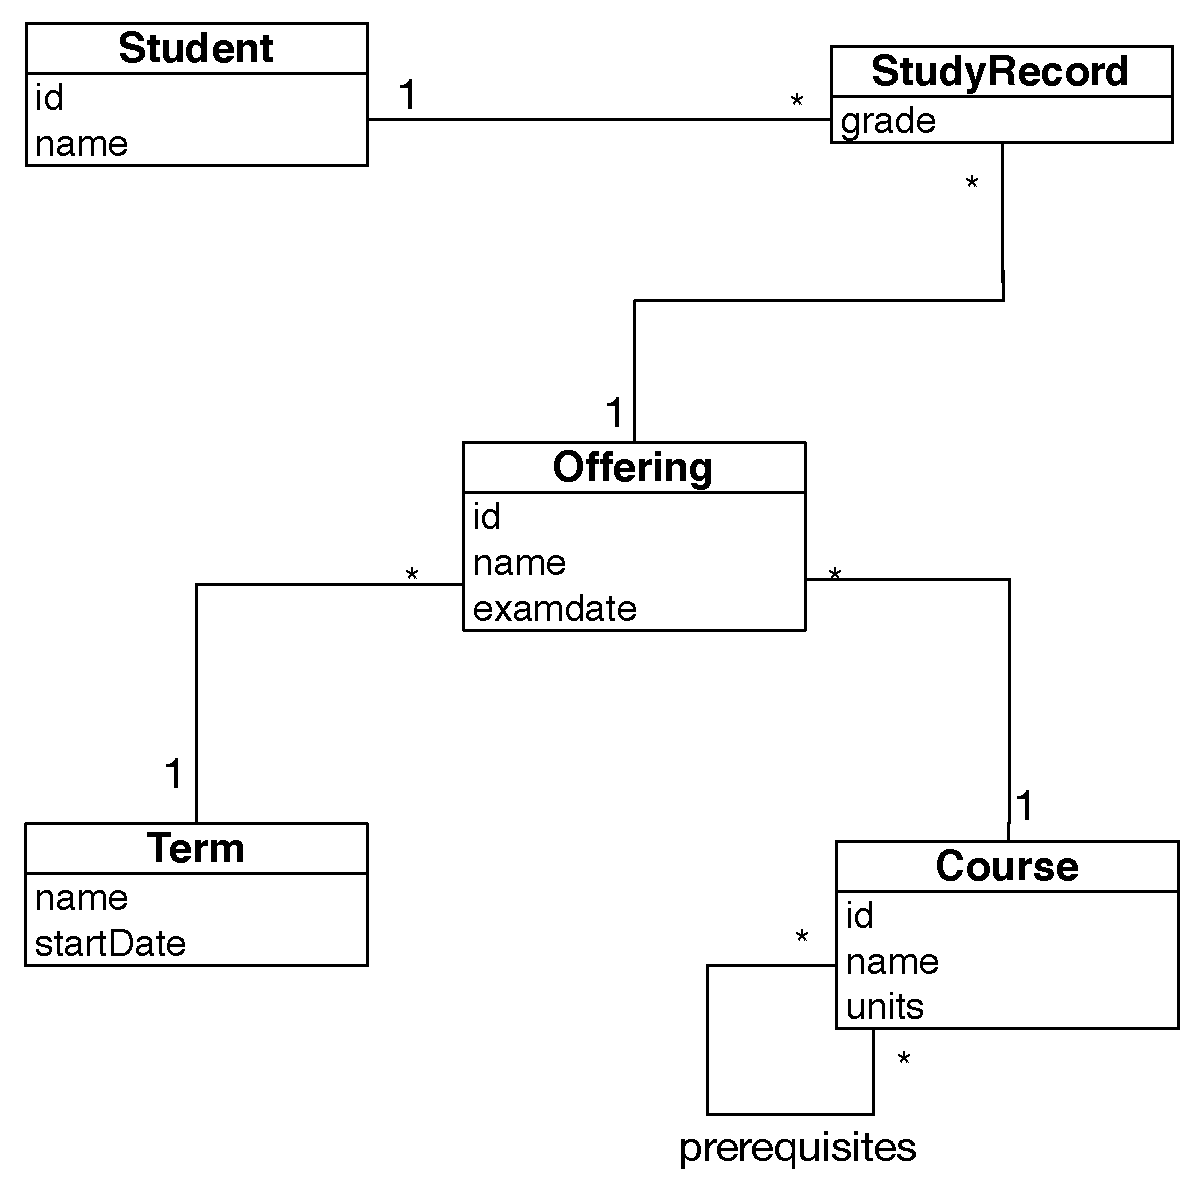
\includegraphics[width=12cm]{4-ProposedFramework/Figures/SimpleClassDiagram.pdf}
    \end{center}
    \caption{\label{fig:edu_class1} نمودار کلاس مدل ابتدای سیستم آموزش ساده }
\end{figure*}
شکل \ref{fig:edu_class1} مدل دامنه‌ی سیستم را به وسیله‌ی یک نمودار کلاس مبتنی بر \textbf{یو‌ام‌ال}\LTRfootnote{UML} نشان می‌دهد.

\newpage
\section{طراحی سیستم آموزش به روش تبادل ناهمگام پیغام}
در این بخش طراحی سیستم معرفی شده در بخش \ref{section:eduIntro} به روش تبادل ناهمگام پیغام ارائه می‌گردد. سعی شده است تا به جای ارائه‌ی یکباره‌ی طراحی نهایی، یک رویکرد \gls{افزایشی}\LTRfootnote{incremental} برای طراحی اتخاذ شود. در این رویکرد مراحل تشکیل نهایی طرح و حتی اقدامات اشتباهی که در طول طراحی برداشته شده است ارائه خواهد شد. به  این ترتیب علاوه بر قابل استفاده‌تر بودن پژوهش به صورت یک دستورالعمل \LTRfootnote{receipe} طراحی، قابلیت فهم روش طراحی هم بالاتر می‌رود.
\subsection{طراحی اکتور‌های مدل دامنه}
اکتورهای اصلی سیستم همان اشیاء مدل دامنه هستند که در بخش \ref{subsec:mainEntities} معرفی شدند.البته احتمالاً علاوه بر این اکتورها، اکتورهای دیگری نیز برای پیاده‌سازی کارکردهای سیستم استفاده خواهند شد. در طراحی اکتورهای اصلی صرفا فیلد‌های داده‌ای اکتور و نیز پیغام‌های اصلی که از روابط موجود در نمودار کلاس \ref{fig:edu_class1} قابل استخراج هستند در نظر گرفته ‌می‌شود. منطق پیاده‌سازی عملیات هر پیغام و  پیغام‌های دیگری که به این منظور ایجاد می‌شوند در ادامه به طراحی افزوده خواهد شد. 
با توجه به اینکه در مدل اکتور،‌ تنها راه ارتباط بین اکتور‌ها استفاده از تبادل پیغام است و این که یک اکتور برای امکان ارسال پیغام به اکتور دیگر نیاز به دسترسی به اسم آن دارد، بهترین راه برای طراحی رابطه‌های وابستگی\LTRfootnote{association} این است که در کلاس یک اکتور برای هر کلاس دیگر که رابطه‌ای با آن وجود دارد یک فیلد از نوع کلاس طرف دیگر در نظر گرفته شود. این مورد مشابه طراحی شیءگرای عادی (ترتیبی) است. از طرف دیگر در مدل طراحی شیءگرای ترتیبی برای هر کارکرد اصلی یک شیء نیز یک متد در کلاس متناظر با آن در نظر گرفته می‌شود که برای اجرای کارکرد، متد مورد نظر فراخوانی می‌شود. با توجه به اینکه در مدل اکتور مکانیزم کنترلی برنامه به جای فراخوانی متد، تبادل پیغام است، باید به ازای هر متد متناظر در حالت شیءگرا، یک پیغام دریافت شود. البته در این مرحله از طراحی منطق پیاده‌سازی کارکرد هر پیغام در نظر گرفته نشده است و در مراحل بعدی به تدریج اضافه خواهد شد.
\begin{enumerate}
%%%%%%%%%%%%%%%%%%%%%%%%%%%%%%%%%
%										Student												%
%%%%%%%%%%%%%%%%%%%%%%%%%%%%%%%%%
\item\textbf{اکتور دانشجو:}
این اکتور دارای فیلد‌های نام و شناسه است. به علت ارتباط دانشجو با سابقه‌ها و نیاز  به ارسال پیغام به آنها یک فیلد از نوع لیست سابقه نیز در کلاس دانشجو وجود دارد. قطعه کد \ref{fig:mainActors:student} طرح ابتدایی کلاس اکتور دانشجو را نشان می‌دهد. همان‌طور که در بخش قبل ذکر شد منطق پیاده‌سازی کارکرد پیغام‌ها در این مرحله اضافه نشده و در ادامه‌ی فصل به تدریج تکمیل خواهد شد. پیغام‌هایی که اکتور دانشجو دریافت می‌کند عبارتند از:
\begin{enumerate}
%\item\textbf{:\lr{HasPassed(course)}}
%با دریافت این پیغام اکتور دانشجو باید پاسخ بدهد که آیا درس مربوطه را گذرانده است یا خیر.
%\item\textbf{:\lr{HasTaken(course)}}
%با دریافت این پیغام دانشجو باید پاسخ دهد که در ترم جاری این درس را اخذ کرده است یا خیر.
\item\textbf{:\lr{GPARequest(term)}}
با دریافت این پیغام دانشجو باید پاسخ دهد که معدل دانشجو در ترم جاری  چند بوده است.
\item\textbf{:\lr{TakeCourse(offering)}}
با دریافت این پیغام دانشجو باید درس ارائه‌ی مربوطه را اخذ کند. طبیعتاً تمام شرایط ذکر شده در مورد کاربرد \ref{table:uc_takecoure} باید بررسی شود.
\end{enumerate}
طبیعتاً این موارد تنها شامل پیغام‌هایی است که مستقیماً از موارد کاربرد قابل استخراج هستند. در هنگام طراحی کارکردهای موارد کاربرد، در صورت لزوم پیغام‌های جدیدی به این کلاس اضافه خواهد شد.
\codelisting[language=scala]{4-ProposedFramework/src/mainActors/Student.scala}{ساختار کلاس اکتور دانشجو}{fig:mainActors:student}
%%%%%%%%%%%%%%%%%%%%%%%%%%%%%%%%%
%										StudyRecord										%
%%%%%%%%%%%%%%%%%%%%%%%%%%%%%%%%%
\item\textbf{اکتور سابقه:}
مطابق مدل دامنه‌ که در شکل \ref{fig:edu_class1} ارائه شده است، تنها فیلد داده‌ای این اکتور، نمره است. به علت ارتباط سابقه با اکتور ارائه، یک فیلد از نوع ارائه نیز در کلاس سابقه وجود دارد. قطعه کد \ref{fig:mainActors:studyrecord} طرح ابتدایی کلاس اکتور سابقه را نشان می‌دهد. همان‌طور که در بخش قبل ذکر شد منطق پیاده‌سازی کارکرد پیغام‌ها در این مرحله اضافه نشده و در ادامه‌ی فصل به تدریج تکمیل خواهد شد. در این مرحله، پیغامی که مستقیماً از موارد کاربرد قابل استخراج باشد وجود ندارد
و در هنگام طراحی کارکردهای موارد کاربرد، در صورت لزوم پیغام‌های جدیدی به این کلاس اضافه خواهد شد.
\codelisting[language=scala]{4-ProposedFramework/src/mainActors/StudyRecord.scala}{ساختار کلاس اکتور سابقه}{fig:mainActors:studyrecord}
%%%%%%%%%%%%%%%%%%%%%%%%%%%%%%%%%
%										Offering										%
%%%%%%%%%%%%%%%%%%%%%%%%%%%%%%%%%
\item\textbf{اکتور ارائه:}
مطابق مدل دامنه‌ که در شکل \ref{fig:edu_class1} ارائه شده است، فیلدهای داده‌ای این اکتور عبارتند از شناسه و تاریخ امتحان\LTRfootnote{examDate}. به علت ارتباط ارائه با اکتور‌های درس و ترم، یک فیلد از نوع درس و یک فیلد از نوع ترم نیز در کلاس ارائه وجود دارد. قطعه کد \ref{fig:mainActors:offering} طرح ابتدایی کلاس اکتور ارائه را نشان می‌دهد. در این مرحله، پیغامی که مستقیماً از موارد کاربرد قابل استخراج باشد وجود ندارد
و در هنگام طراحی کارکردهای موارد کاربرد، در صورت لزوم پیغام‌های جدیدی به این کلاس اضافه خواهد شد.
\codelisting[language=scala]{4-ProposedFramework/src/mainActors/Offering.scala}{ساختار کلاس اکتور ارائه}{fig:mainActors:offering}



%%%%%%%%%%%%%%%%%%%%%%%%%%%%%%%%%
%										Course										%
%%%%%%%%%%%%%%%%%%%%%%%%%%%%%%%%%
\item\textbf{اکتور درس:}
مطابق مدل دامنه‌ که در شکل \ref{fig:edu_class1} ارائه شده است، فیلدهای داده‌ای این اکتور عبارتند از شناسه، نام و تعداد واحد. تنها ارتباط این کلاس که نیاز به ایجاد فیلد دارد ارتباط دروس پیش‌نیاز است. بنابراین یک فیلد از نوع لیست درس نیز به این منظور باید به کلاس اضافه شود. قطعه کد \ref{fig:mainActors:course} طرح ابتدایی کلاس اکتور درس را نشان می‌دهد. در این مرحله، پیغامی که مستقیماً از موارد کاربرد قابل استخراج باشد وجود ندارد
و در هنگام طراحی کارکردهای موارد کاربرد، در صورت لزوم پیغام‌های جدیدی به این کلاس اضافه خواهد شد.
\codelisting[language=scala]{4-ProposedFramework/src/mainActors/Course.scala}{ساختار کلاس اکتور درس}{fig:mainActors:course}
%%%%%%%%%%%%%%%%%%%%%%%%%%%%%%%%%
%										Term										%
%%%%%%%%%%%%%%%%%%%%%%%%%%%%%%%%%
\item\textbf{اکتور ترم:}
مطابق مدل دامنه‌ که در شکل \ref{fig:edu_class1} ارائه شده است، فیلدهای داده‌ای این اکتور عبارتند از نام و تاریخ شروع{startDate}. با توجه به موارد کاربرد مطرح شده، اکتور ترم آغاز کننده‌ی هیچ ارتباطی نیست و به همین دلیل نیازی به داشتن فیلدی برای این منظور نیست. اکتور ترم قطعه کد \ref{fig:mainActors:term} طرح ابتدایی کلاس اکتور ترم را نشان می‌دهد. در این مرحله، پیغامی که مستقیماً از موارد کاربرد قابل استخراج باشد وجود ندارد
و در هنگام طراحی کارکردهای موارد کاربرد، در صورت لزوم پیغام‌های جدیدی به این کلاس اضافه خواهد شد.
\codelisting[language=scala]{4-ProposedFramework/src/mainActors/Term.scala}{ساختار کلاس اکتور ترم}{fig:mainActors:term}
\end{enumerate}
\newpage
\subsection{مورد کاربرد محاسبه‌ی معدل}
این مورد کاربرد در جدول \ref{table:uc_gpa} توصیف شده است. 
\subsubsection{رویکرد اول}
\label{gpa_approach1}
برای محاسبه‌ی معدل ترم یک دانشجو نیاز داریم نمره‌ی تمام درس‌های دانشجو در ترم به همراه تعداد واحد‌های آن درس‌ها را در اختیار داشته باشیم. درخواست معدل برای ترم از طرف دانشجو صورت می‌گیرد بنابراین شروع پیغام‌ها از این اکتور آغاز می‌شود.
 اکتور دانشجو به هر کدام از اکتور‌های سابقه\LTRfootnote{StudyRecord} یک پیغام می‌فرستد و به وسیله‌ی آن اعلام می‌کند نمره و تعداد واحد‌های درس مربوط به سابقه در پاسخ ارسال شود. علاوه بر این، در پاسخ باید مشخص شود که آیا سابقه‌ مربوط به همان ترم است که معدل برای آن درخواست شده یا خیر. بنابراین پیغام‌های  درخواست نمره برای معدل و پاسخ آن به صورت زیر خواهند بود:
\begin{latin}
 \begin{description}
 \item[\lr{request: GPAInfoRequest( term: Term)}]
  \item[\lr{response: GPAInfoResponse(isForTerm:Boolean, grade: Double, units:Int)}]
 \end{description}
 \end{latin}
  اکتور سابقه امکان اینکه بدون برقراری ارتباط با اکتور ارائه\LTRfootnote{Offering} جواب این پیغام را بدهد، ندارد. دلیل این امر این است که اولا سابقه‌ لزوما مربوط به ترمی نیست که معدل برای آن درخواست شده است، ثانیا سابقه اطلاعی از تعداد واحد‌های درس مربوطه ندارد. به همین دلیل، سابقه باید برای جمع‌آوری این اطلاعات با اکتورهای دیگر تبادل پیغام انجام دهد. از طرف دیگر تنها اکتوری که به نمره‌ی دانشجو دسترسی ادارد، اکتور سابقه است. در نتیجه فرستادن پاسخ به درخواست دانشجو نیاز به همکاری ۳ اکتور سابقه، درس و ترم دارد. با توجه به اینکه دسترسی سابقه به اکتورهای درس و ترم از طریق اکتور ارائه ممکن می‌شود، این اکتور نیز در تبادل پیغام‌ها مشارکت خواهد داشت.\\
با توجه به موارد ذکر شده، اکتور سابقه دو راهکار پیش رو دارد:
\begin{enumerate}
\item اکتور سابقه به وسیله‌ی درخواست‌هایی، تعیین کند که ترم مربوط به این سابقه همان ترم مورد درخواست در معدل است یا خیر، و نیز تعداد واحد‌های درس چند است. و  در ادامه با ترکیب این اطلاعات با نمره‌ی سابقه، خود پاسخ اکتور دانشجو را ارسال کند.
\item اکتور سابقه نمره را در پاسخ قرار دهد ولی با توجه به اینکه پاسخ هنوز کامل نیست (هنوز معلوم نیست که درس چند واحدی است و آیا مربوط به ترم درخواستی است یا خیر)، به جای اینکه پاسخ را برای دانشجو پس بفرستد، آن را برای تکمیل به اکتور ارائه منتقل کند.
\end{enumerate} 
در این رویکرد فرض بر انتخاب اول است، یعنی اینکه خود اکتور سابقه، با گرفتن اطلاعات مورد نیاز از ارائه، پاسخ دانشجو را ارسال می‌کند.\\
برای این کار اکتور سابقه پیغام GPAInfoRequest را برای اکتور ارائه ارسال می‌کند و منتظر دریافت پاسخ می‌ماند. اکتور ارائه با دریافت GPAInfoRequest دو پیغام به صورت زیر به ترتیب برای اکتور ترم و اکتور درس ارسال می‌کند و منتظر پاسخ آنها می‌ماند:
\begin{latin}
 \begin{description}
 \item[\lr{IsYourTermRequest(term: Term)}]
  \item[\lr{NumOfUnitsRequest}]
 \end{description}
 \end{latin}
هدف از درخواست اول این است که مشخص شود که  درسی که سابقه به آن متعلق است، متعلق به همان ترمی است که معدل برای‌ آن درخواست شده یا خیر (اگر جواب خیر باشد نمره‌ی درس در معدل در نظر گرفته نخواهد شد). پیغام دوم هم تعداد واحد‌های درس را از اکتور درس درخواست می‌کند. ترم و درس به سادگی به این دو پیغام پاسخ می‌دهند و ارائه با گرفتن پاسخ‌ها، اطلاعات آنها را تجمیع\footnote{منظور از تجمیع در اینجا این است که  پاسخ فرضی true برای پیغام \lr{IsYourTermRequest(term)} و پاسخ فرضی 3 برای پیغام \lr{NumOfUnitsRequest} را که به ترتیب از اکتورهای ترم و درس گرفته شده، به صورت پیغام \lr{GPAInfoResponse(isForTerm=true,grade=null,unit=3)} باهم ترکیب می‌کند.} کرده و برای اکتور سابقه ارسال می‌کند.  سابقه با دریافت این پیغام، به تمام اطلاعات لازم برای این که پاسخ اکتور دانشجو را بدهد، دسترسی دارد. بنابراین می‌تواند با اضافه کردن مقدار فیلد نمره‌ی خود به پیغام آن را برای دانشجو ارسال کند. دانشجو با گرفتن این پاسخ، یکی از نمره‌های لازم برای محاسبه‌ی معدل را در دست دارد. بقیه‌ی نمره‌ها از تکرار همین عملیات برای تمام اکتورهای سابقه‌ی مربوط به دانشجو به طور مشابه به دست می‌آیند. در نهایت اکتور دانشجو با جمع نمراتی که مربوط به ترم درخواستی بوده‌اند (که از مقدار فیلد isForTerm از پیغام‌های پاسخ قابل تشخیص است) و تقسیم آن بر جمع واحد‌های مربوط به ترم (فیلد units پیغام پاسخ) معدل را محاسبه کرده و برای اکتوری که درخواست معدل داده ارسال می‌کند.
   شکل \ref{fig:gpa1_sequence} نمودار ترتیب\LTRfootnote{sequence diagram} برای پیغام‌های مبادله شده در این رویکرد را در قالب یک مثال نشان می‌دهد. در بخشی از این مثال که در شکل قابل مشاهده است فرض شده ترم مربوط به درخواست معدل باشد و تعداد واحد‌های درس ۳ باشد. نمره‌ی سابقه‌ای که درخواست برای آن ارسال شده ۱۲ است. درنهایت پس از تکرار حلقه‌ی مشخص شده در شکل و ارسال پیغام‌‌ها به تمام سابقه‌ها عدد فرضی ۱۵/۲۵ به عنوان معدل محاسبه شده و به صورت پیغام ارسال شده است. لازم به ذکر است که در این شکل برای سادگی نمایش فرض شده که تکرارهای حلقه برای سابقه‌های مختلف انجام شده است و طبیعتا استاندارد یو‌ام‌ال برای آن به طور کامل رعایت نشده است.

\begin{figure*}
    \begin{center}
	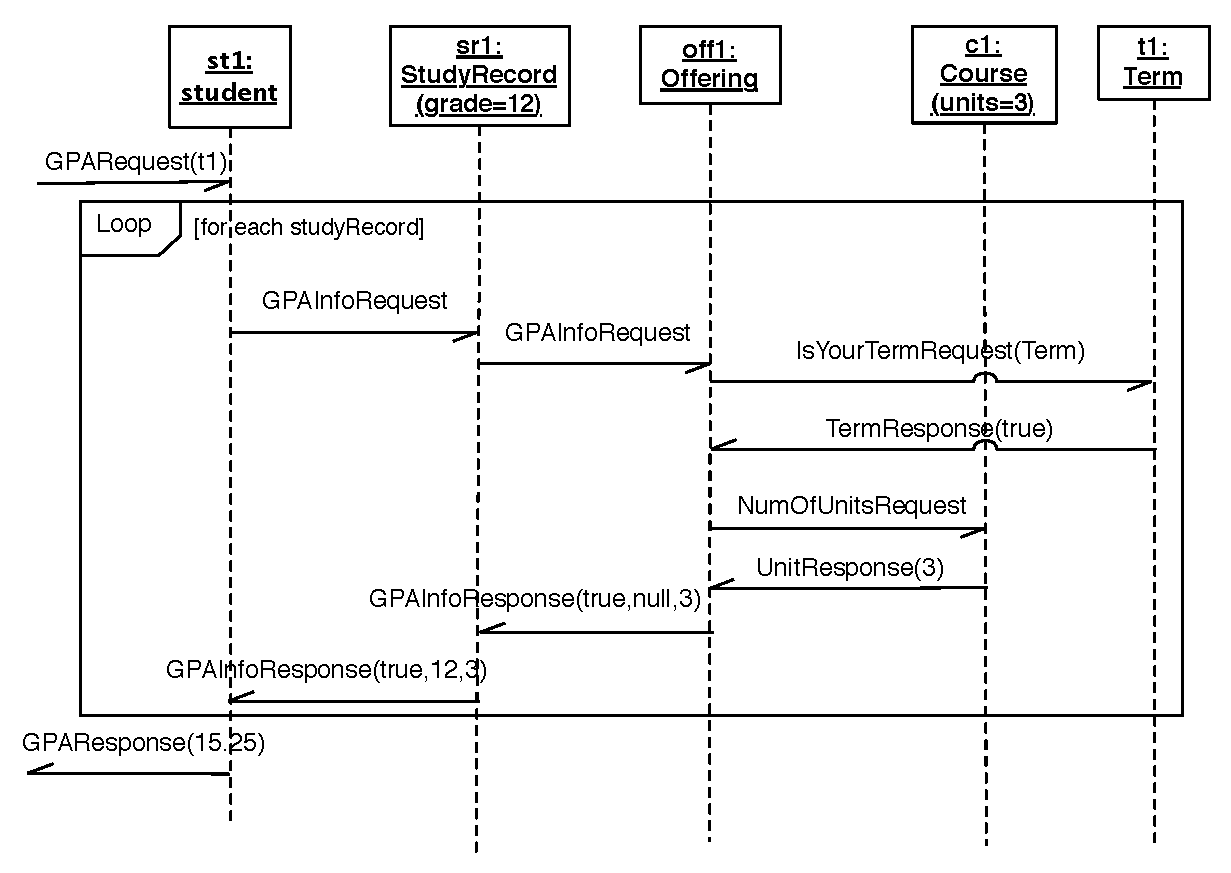
\includegraphics[width=16cm]{4-ProposedFramework/Figures/gpa_1_sequence.pdf}
    \end{center}
    \caption{\label{fig:gpa1_sequence} نمودار ترتیب برای رویکرد اول محاسبه‌ی معدل }
\end{figure*}
\FloatBarrier
در این بخش از طراحی لازم است به دو پرسش مهم پاسخ دهیم:\\
پرسش اول این است که در هر کدام از قسمت‌های طراحی که یک اکتور پیغام را فرستاده و منتظر جواب می‌ماند، آیا اکتور می‌تواند در طول مدت انتظار به فعالیت‌های دیگربپردازد؟ به عبارت بهتر، \textbf{آیا ارسال پیغام‌ها به صورت همگام است یا ناهمگام؟}\\
پرسش دوم این است که در صورتی که ارسال پیغام ناهمگام باشد ادامه‌ی فعالیت اکتور به چه صورتی مجاز است؟ آیا می‌تواند پیغام‌های جدیدی دریافت کند و به اجرای منطق مربوط به آنها بپردازد؟\\
برای پاسخ به این پرسش‌ها در رویکرد اول، در هر مورد که پیغامی دریافت و فرستاده می‌شود این پرسش‌ها را بررسی می‌کنیم:
\begin{enumerate}
\item اکتور دانشجو:\\
تنها پیغامی که اکتور دانشجو تا این مرحله از طراحی ارسال می‌کند پیغام GPAInfoRequest است. ابتدا منطق پیاده‌سازی شده در این تبادل این پیغام را بررسی ‌می‌کنیم:\\
 شبه کد \ref{fig:usecases:gpa:1:student_sync} تبادل پیغام‌های دانشجو با اکتور‌های سابقه را نشان می‌دهد. در این قطعه‌کد از دستور \lr{?!} (تبادل همگام) برای فرستادن پیغام استفاده شده است. اکتور دانشجو به هر اکتور سابقه یک پیغام GPAInfoRequest می‌فرستد و با دریافت هر پاسخ GPAInfoResponse این عملیات را انجام می‌دهد:
در صورتی که فیلد isForTerm از پیغام مقدار true داشته باشد مجموع وزن‌دار\footnote{عددی که از جمع حاصل‌ضرب هر نمره در تعداد واحدهای درس حاصل شده است.} نمرات گرفته شده تا حال را با حاصل ضرب فیلد grade در فیلد units جمع می‌کند. و حاصل جمع واحد‌ها را به اندازه‌ی units افزایش می‌دهد. نهایتا بعد از مبادله‌ی پیغام با تمام اکتور‌های سابقه، حاصل تقسیم  مجموع وزن‌دار نمرات بر تعداد واحد‌ها به عنوان معدل دانشجو در ترم اعلام می‌شود.
\codelisting[language=scala]{4-ProposedFramework/src/usecases/gpa/1/Student_sync.scala}{شبه‌کد اسکالا برای اکتور دانشجو در رویکرد ۱ با ارسال همگام پیغام}{fig:usecases:gpa:1:student_sync} 

حال پرسش اول برای اکتور دانشجو به این صورت بیان می‌شود:\\
آیا اکتور دانشجو بعد از ارسال پیغام GPAInfoRequest به یک اکتور سابقه و در مدتی که هنوز پاسخی از این اکتور دریافت نکرده می‌تواند به فعالیت خود ادامه دهد؟ ابتدا باید به این نکته دقت کرد که تفاوت اصلی رویکرد حاصل از پاسخ مثبت به این پرسش (ارسال ناهمگام) و پاسخ منفی به آن (ارسال همگام) از دیدگاه اکتور فرستنده‌ی درخواست چیست؟ با کمی دقت و تحلیل می‌توان دریافت که تفاوت اصلی این دو رویکرد از دیدگاه فرستنده در نحوه‌ی برخورد با پاسخ پیغام است. به بیان دقیق‌تر در حالت همگام، این که پاسخ دریافت شده مربوط به کدام درخواست بوده است، به طور ضمنی مشخص است. ولی اگر بعد از ارسال پیغام، اکتور منتظر جواب نماند و به کار خود ادامه دهد در هر زمان دیگری ممکن است پاسخ دریافت شود و در این هنگام امکان اینکه تشخیص داده شود این پاسخ مربوط به کدام درخواست بوده ممکن است امکان‌پذیر نباشد. دقت به منطق پیاده شده برای دریافت پیغام GPAInfoResponse نشان می‌دهد که اینکه هر پاسخ مربوط به کدام درخواست بوده اهمیتی ندارد. به بیان دیگر ترتیب دریافت این پاسخ‌ها تاثیری در معدل اعلام شده ندارد. بنابراین پاسخ به پرسش اول در مورد اکتور دانشجو مثبت است. \\
\textbf{نتیجه:}
می‌توانیم پیغام‌های GPAInfoRequest را به صورت ناهمگام ارسال کنیم.\\
اکنون نوبت به پرسش دوم می‌رسد: آیا اکتور دانشجو در حالی که هنوز پاسخ تمام پیغام‌ها را دریافت نکرده می‌تواند درخواست جدیدی را پردازش کند؟\\
برای پاسخ به این پرسش فرض می‌کنیم که اکتور دانشجو در حالی که پاسخ تعدادی از پیغام‌های GPAInfoRequest را دریافت نکرده، یک پیغام جدید \lr{GPARequest} دریافت می‌کند (یک درخواست جدید برای محاسبه‌ی معدل). برای محاسبه‌ی معدل، اکتور دانشجو مطابق منطق پیاده شده اقدام به ارسال پیغام GPAInfoRequest به تمام اکتور‌های سابقه می‌کند. در این حالت فرض کنیم یک پیغام پاسخ GPAInfoResponse دریافت شود. با دریافت این پیغام باید متغیرهای محلی اکتور دانشجو به هدف محاسبه‌ی معدل بروزرسانی می‌شوند. اما با توجه به اینکه مشخص نیست که پاسخ دریافت شده مربوط به کدام در خواست بوده است نمی‌توانیم معدل را به صورت صحیح محاسبه کنیم. به عبارت دیگر منطق محاسبه‌ی معدل برای دو درخواست باهم مخلوط می‌شوند. به همین دلیل پاسخ به پرسش دوم منفی است.\\
\textbf{نتیجه:}
علیرغم اینکه ارسال پیغام‌های GPAInfoRequest را می‌توانیم به صورت ناهمگام انجام دهیم (چون ترتیب دریافت پیغام‌ها اهمیتی ندارد)، قبل از دریافت همه‌ی پاسخ‌های مربوط به درخواست معدل درحال پردازش، نمی‌توانیم درخواست جدیدی دریافت کنیم.\\
البته باید دقت کرد که با وجود اینکه میزان به تعویق انداختن دریافت پاسخ‌ها محدود است (به دلیل پرسش دوم)، کماکان ارسال ناهمگام پیغام‌های  GPAInfoRequest ارزشمند است. چرا که در حالت تبادل ناهمگام، تمام اکتورهای سابقه، به صورت همروند پاسخ این پیغام را آماده می‌کنند در حالی که در حالت همگام به صورت نوبتی و ترتیبی این اتفاق می‌افتد.\\
با توجه به پاسخ به این دو پرسش، طراحی اکتور دانشجو برای محاسبه‌ی معدل به صورت شبه‌کد شکل \ref{fig:usecases:gpa:1:student_Async} تغییر می‌کند. در این شبه‌کد از روش تبادل پیغام  \gls{آینده}\LTRfootnote{Future} (رجوع کنید به بخش \ref{section:scalaActorLib}) استفاده شده است.

\codelisting[language=scala]{4-ProposedFramework/src/usecases/gpa/1/Student_Async.scala}{شبه‌کد اسکالا برای اکتور دانشجو در رویکرد ۱ با ارسال ناهمگام پیغام (آینده)}{fig:usecases:gpa:1:student_Async} 

 \FloatBarrier
% در واقع این حالت، رویکرد پیش‌فرض در طراحی به روش شیءگرا است. ارسال پیغام همگام در مدل اکتور در واقع معادل با فراخوانی یک متد در مدل شیءگرای ترتیبی است. و این خاصیت طراحی ترتیبی زیربنای نحوه‌ی استدلال در مورد طرز کار طراحی است. در طراحی ترتیبی اطمینان داریم که تفاوت حالت شیء قبل از  فراخوانی یک متد و بعد از آن، صرفا به منطق پیاده شده در داخل متد وابسته است و خارج از آن هیچ تغییر دیگری رخ نخواهد داد. در صورتی که در طراحی همروند به صورت ناهمگام، این‌گونه نیست.
\item اکتور سابقه:\\
در مورد اکتور سابقه جواب دادن به ۲ پرسش مذکور آسان‌تر است. این اکتور فقط پیغام GPAInfoRequest را ارسال می‌کند و با دریافت هر پیغام پاسخ GPAInfoResponse، صرفا نمره‌ی سابقه را به آن اضافه کرده و برای اکتور دانشجو ارسال می‌کند. واضح است که در این تبادل پیغام، ترتیب پیغام‌‌های پاسخ اهمیتی ندارد. بنابراین پاسخ اولین پرسش مثبت است (ارسال ناهمگام مجاز است). در مورد پرسش دوم با اینکه این اکتور هیچ حالتی\LTRfootnote{state} برای درخواست‌ها نگه نمی‌دارد.\footnote{بر خلاف حالت اکتور دانشجو که در آن متغیر‌هایی برای هر درخواست مقداردهی می‌شدند.} اما دریافت درخواست جدید قبل از گرفتن پاسخ‌های درخواست قبلی  مشکل دیگری ایجاد می‌کند. با توجه به اینکه  هر درخواست که از اکتور دانشجو به اکتور سابقه می‌رسد، نهایتا باید توسط خود اکتور سابقه پاسخ داده شود، در هنگام فرستادن پیغام پاسخ باید آدرس فرستنده‌ی درخواست اولیه موجود باشد. در حالی که اگر قبل از پاسخ به درخواست اکتور دانشجو، درخواست جدیدی دریافت شود و عملیات پردازش درخواست جدید آغاز گردد، هیچ اثری از فرستنده‌ی 
درخواست اول برای ارسال پاسخ به آن موجود نخواهد بود. برای روشن شدن مطلب، شبه‌کد  \ref{fig:usecases:gpa:1:studyrec_Async_wrong} را در نظر بگیرید که در آن فرض شده اکتور سابقه بتواند قبل از فرستادن پاسخ درخواست قبلی، درخواست جدیدی را پردازش کند. همان‌طور که در خط ۱۱ کد اشاره شده است، در هنگامی‌که یک پاسخ از اکتور ارائه دریافت شده، دسترسی به اکتور فرستنده‌ی پیغام اصلی (که در خط ۸ دریافت شده) وجود ندارد تا بتوانیم پاسخ را برای آن ارسال کنیم. باید دقت شود که با اینکه فرستنده‌ی یک پیغام به وسیله‌ی شیء sender قابل دسترسی است، اما این شیء به فرستنده‌ی پیغامی اشاره می‌کند که پیغام آن در حال پردازش است. در مورد خط ۱۱ این شیء اشاره به اکتور ارائه دارد که فرستنده‌ی آخرین پیغام بوده، نه اکتور دانشجو که در انتظار گرفتن پاسخ از اکتور سابقه است. بنابراین پاسخ به پرسش دوم در مورد اکتور سابقه منفی است و این اکتور باید پاسخ هر درخواست را قبل از  پردازش درخواست‌های دیگر ارسال کند. نکته‌ی قابل توجه این است که با توجه به اینکه اکتور سابقه برای پاسخ به درخواست GPAInfoRequest تنها یک پیغام ارسال می‌کند و بدون دریافت پاسخ آن قادر به پاسخگویی به درخواست مذکور نیست، تفاوتی در ارسال همگام و ناهمگام پیغام وجود ندارد چرا که پس از ارسال تنها یک پیغام مجبور به توقف و انتظار برای دریافت پاسخ است. شبه کد \ref{fig:usecases:gpa:1:studyrec_Async_right} طراحی صحیح تبادل پیغام در اکتور سابقه را برای رویکرد ۱ نشان می‌دهد.

\codelisting[language=scala]{4-ProposedFramework/src/usecases/gpa/1/StudyRecord_Async_wrong.scala}{شبه‌کد اکتور سابقه برای حالتی که بتواند قبل از پاسخ به درخواست قبلی، درخواست جدیدی را پردازش کند. (این رویکرد اشتباه است.)}{fig:usecases:gpa:1:studyrec_Async_wrong} 

\codelisting[language=scala]{4-ProposedFramework/src/usecases/gpa/1/StudyRecord_Async_right.scala}{شبه‌کد صحیح برای  اکتور سابقه در رویکرد ۱}{fig:usecases:gpa:1:studyrec_Async_right} 

\FloatBarrier
\item اکتور ارائه:\\
اکتور ارائه پس از دریافت درخواست GPAInfoRequest دو پیغام به ترتیب برای اکتور‌های ترم و درس ارسال می‌کند و در هر کدام از این دو پیغام بخشی از اطلاعات لازم برای فرستادن پاسخ به اکتور سابقه را از آنها دریافت می‌کند.
پرسش اول در مورد اکتور ارائه اینطور مطرح می‌شود که آیا اکتور ارائه پس از فرستادن هر کدام از پیغام‌های مذکور به ترم و درس می‌تواند پیغام بعدی را ارسال کند یا باید پس از ارسال هرکدام بلافاصله منتظر دریافت پاسخ بماند؟ جواب این پرسش مثبت است به این دلیل که ترتیب پیغام‌های پاسخ اهمیتی ندارد. اما با استدلالی مشابه آنچه که در مورد اکتور سابقه توضیح داده شد، جواب پرسش دوم برای اکتور ارائه منفی است. یعنی اکتور ارائه تا زمانی که پاسخ یک درخواست را به اکتور سابقه‌ی مربوطه نفرستاده، نمی‌تواند درخواست جدیدی (احتمالاً از یک اکتور سابقه‌ی دیگر) پردازش کند. به همین دلیل حداکثر میزان ناهمگامی در ارسال پیغام‌ها برای اکتور ارائه این است که دو پیغام IsYourTermRequest و  NumOfUnitsRequest را به صورت ناهمگام برای اکتورهای ترم و درس ارسال کند و سپس منتظر دریافت پاسخ آنها بماند. بنابراین طراحی تبادل پیغام اکتور ارائه در رویکرد ۱ مطابق شبه‌کد شکل \ref{fig:usecases:gpa:1:offering_Async_right}  خواهد بود. در این شکل نیز از ویژگی آینده\LTRfootnote{Future} (رجوع کنید به \ref{section:scalaActorLib}) استفاده شده است.
\codelisting[language=scala]{4-ProposedFramework/src/usecases/gpa/1/Offering_Async_right.scala}{شبه‌کد طراحی نحوه‌ی تبادل پیغام برای  اکتور ارائه در رویکرد ۱.}{fig:usecases:gpa:1:offering_Async_right} 
\FloatBarrier
\item اکتورهای ترم و درس:\\
در مورد  این دو اکتور تصمیم به استفاده از ارسال همگام یا ناهمگام بسیار ساده است. با توجه به اینکه در هر دو اکتور مذکور، تمام اطلاعات لازم برای پاسخ به درخواست‌ها در خود اکتور موجود است، نیازی به ارسال پیغام به سایر اکتورها وجود ندارد و پاسخ درخواست‌ها بلافاصله ارسال می‌شود. لذا هیچ نیازی به تبادل همگام وجود ندارد (چون پاسخی دریافت نخواهد شد). طراحی این دو اکتور از نظر تبادل پیغام در شبه‌کدهای \ref{fig:usecases:gpa:1:term}  و \ref{fig:usecases:gpa:1:course}  نمایش داده شده است.
\codelisting[language=scala]{4-ProposedFramework/src/usecases/gpa/1/Term.scala}{شبه‌کد طراحی نحوه‌ی تبادل پیغام برای  اکتور ترم در رویکرد ۱.}{fig:usecases:gpa:1:term} 
\codelisting[language=scala]{4-ProposedFramework/src/usecases/gpa/1/Course.scala}{شبه‌کد طراحی نحوه‌ی تبادل پیغام برای  اکتور درس در رویکرد ۱.}{fig:usecases:gpa:1:course} 
\FloatBarrier

\end{enumerate}

\subsubsection{رویکرد دوم}
\label{gpa_approch2}
رویکرد دوم از طراحی مورد کاربرد محاسبه‌ی مدل را با بررسی رویکرد ۱ و طرح چند پرسش در مورد آن آغاز می‌کنیم. نحوه‌ی طراحی ارتباطات و پیغام‌ها در رویکرد اول در بخش قبل به طور کامل توضیح داده شد. در این قسمت خلاصه‌ای از این طراحی را بررسی می‌کنیم:\\
عملیات با دریافت پیغام درخواست معدل \lr{GPARequest(term)} در اکتور دانشجو آغاز می‌شود. اکتور دانشجو به هر کدام از اکتورهای سابقه، یک پیغام درخواست اطلاعات معدل \lr{GPAInfoRequest(term)} ارسال می‌کند. این پیغام از طریق اکتور سابقه به دست اکتور ارائه می‌رسد و از طریق این اکتور به دست اکتورهای درس و ترم می‌رسد و هر کدام از این اکتورها اطلاعات لازم را برای اکتور ارائه ارسال می‌کنند. در ادامه اکتور ارائه یک پیغام پاسخ اطلاعات معدل \lr{(GPAInfoResponse)}  تولید می‌کند و برای اکتور سابقه ارسال می‌کند. سابقه عدد نمره را به پیغام اضافه کرده و برای دانشجو می‌فرستد. دانشجو با تکرار همین عملیات برای تمام سابقه‌ها تمام اطلاعات لازم برای محاسبه‌ی معدل در اختیار دارد.\\
هر اکتور در این مورد کاربرد به دلایل مختلفی اقدام به مشارکت در محاسبه‌ی معدل می‌کند: دانشجو به این دلیل که مسئولیتِ گرفتن درخواست اصلی را دارد و نیز به این دلیل که به اکتور سابقه دسترسی دارد. اکتور سابقه به این دلیل که نمره (یکی از اطلاعات لازم برای محاسبه‌ی معدل) را در اختیار دارد و نیز از طریق اکتور ارائه به درس و ترم دسترسی دارد. اکتور ارائه به دلیل دسترسی به درس و ترم. و اکتورهای درس و ترم به دلیل اینکه اطلاعات مورد نیاز برای محاسبه‌ی معدل را در اختیار دارند. در نتیجه مشارکت تمام این اکتورها در محاسبه‌ی معدل ضروری است. اما پرسشی که پیش می‌آید این است که آیا میزان مشارکت این اکتورها نیز باید در همین میزان باشد؟ اگر هر دریافت یا ارسال یک نوع پیغام را یک مشارکت برای اکتور در طراحی این مورد کاربرد در نظر بگیریم، آیا می‌توان تعداد مشارکت‌های اکتورها را کاهش داد؟ به عنوان مثال اکتور سابقه را در نظر می‌گیریرم. همان‌طور که ذکر شد مشارکت این اکتور به دلیل داشتن فیلد نمره و نیز دسترسی به اکتور ارائه ضروری است. تعداد مشارکت اکتور  سابقه با توجه به تعریف ارائه شده، از روی نمودار ترتیب شکل \ref{fig:gpa1_sequence} به این ترتیب قابل استخراج است: هر فلشی که از خط زمان\LTRfootnote{time line} اکتور سابقه خارج یا به آن وارد می‌شود معادل ارسال یا دریافت یک نوع پیغام است. بنابراین تعداد مشارکت اکتور سابقه در این مورد کاربرد ۴ است. مشارکت اول مربوط به دریافت پیغامِ درخواست از دانشجو است، مشارکت دوم مربوط به ارسال درخواست به ارائه است، مشارکت سوم دریافت پاسخ از ارائه و مشارکت چهارم مربوط به ارسال پاسخ به دانشجو است. حال بررسی می‌کنیم که از این تعداد مشارکت، دو مورد الزامی است. یکی دریافت درخواست از دانشجو به دلیل اینکه دانشجو از طریق دیگری به اطلاعات مورد نیاز برای محاسبه‌ی معدل دسترسی ندارد، و دیگری ارسال درخواست برای ارائه. دو مورد دیگر یعنی دریافت پاسخ ارائه و تحویل آن به دانشجو را می‌توان حذف کرد. روش حذف به این صورت است که اکتور ارائه به نحوی مطلع شود که جواب نهایی به چه کسی ارسال خواهد شد (دانشجو). این کار از طریق \textbf{قرار دادن مقصد نهایی پیغام در داخل پیغام} قابل انجام است. در این حالت دیگر نیازی به برگشت پیغام به دست سابقه وجود ندارد. تنها موردی که موردی که به نظر مشکل‌ساز می‌آید این است که فیلد نمره در رویکرد ۱ در هنگام برگشت پیغام در  آن قرار داده می‌شود و اگر پیغام از طریق سابقه برگشت داده نشود فیلد نمره را نخواهد داشت. البته این مورد به سادگی قابل حل است و در همان بار اول که پیغام به دست سابقه رسید، می‌تواند نمره را به پیغام اضافه کند. البته مثال اکتور سابقه در مورد بقیه‌ی اکتورها نیز قابل بررسی است ولی به دلیل پرهیز از تکرار استدلال به همین مورد اکتفا می‌کنیم.\\
مورد دیگری که در رویکرد ۱ بررسی می‌کنیم عدم امکان پردازش درخواست‌های جدید در هنگام انتظار برای تکمیل اطلاعات مورد نیاز برای پاسخ به درخواست قبلی است. مثلا در مورد دانشجو این مورد باعث شد که در رویکرد ۱، دانشجو قبل از ارسال پاسخ درخواست معدل،‌ درخواست دیگری را بررسی کند. در مورد دانشجو دلیل این پدیده این بود که منطق محاسبه‌ی معدل قسمتی از حالت\LTRfootnote{state} این اکتور بود و تداخل درخواست‌های معدل می‌تواند باعث عملکرد غلط اکتور شود. یک راه برای حل این مشکل این است که به نوعی مشخص کنیم که هر پاسخی که اکتور دانشجو دریافت می‌کند مربوط به کدام درخواست اصلی بوده‌ است. یعنی حالت اکتور را در قالب نگاشت‌هایی از پیغام‌ها حفظ کنیم. مثلا برای اکتور دانشجو، به جای اینکه یک متغیر برای مجموع نمره‌هایی که تا این لحظه پاسخ آنها بررسی شده (رجوع کنید به شبه‌کد شکل \ref{fig:usecases:gpa:1:student_Async})، می‌توانیم نگاشتی\LTRfootnote{map} از شناسه‌ی درخواست معدل به متغیر مجموع نگهداری کنیم، به این ترتیب با رسیدن یک پاسخ، متغیر مربوط به درخواست مربوطه برای محاسبه استفاده می‌شود. البته این روش اولاً باعث پیچیده‌تر شدن منطق اکتور می‌شود و ثانیاً نگهداری ساختار داده‌ی نگاشت اهمیت زیادی پیدا می‌کند. به این دلایل استفاده از نگاشت رویکرد مناسبی نیست. روش دیگر این است که به حالت مربوط به بررسی یک درخواست را به اکتور دیگری که به همین منظور ایجاد می‌شود، منتقل کنیم. مثلا وقتی دانشجو یک درخواست محاسبه‌ی معدل دریافت می‌کند، یک اکتور مختص همان درخواست ایجاد کنیم و همه‌ی تبادلات مربوط به آن درخواست را به اکتور جدید واگذار کنیم. طبیعتا تمام اطلاعات لازم از جمله دسترسی به اکتور سابقه باید به اکتور جدید منتقل شود. در نتیجه‌ی این رویکرد، دانشجو می‌تواند با دریافت هر درخواست معدل بلافاصله به پردازش آن بپردازد.\\
با توجه به موارد ذکر شده و بدون تکرار نکاتی که در رویکرد اول ذکر شد به ارائه‌ی خلاصه‌ای از طراحی اکتورها در رویکرد دوم می‌پردازیم.
شکل \ref{fig:gpa2_sequence} نمودار ترتیب برای رویکرد دوم محاسبه‌ی معدل را نشان ‌می‌دهد. برای پرهیز از تکرار، در این رویکرد مراحل طراحی معرفی شده در رویکرد اول بسط داده نشده است و صرفاً چند تغییر اساسی توضیح داده می‌شود.

\begin{figure*}
    \begin{center}
	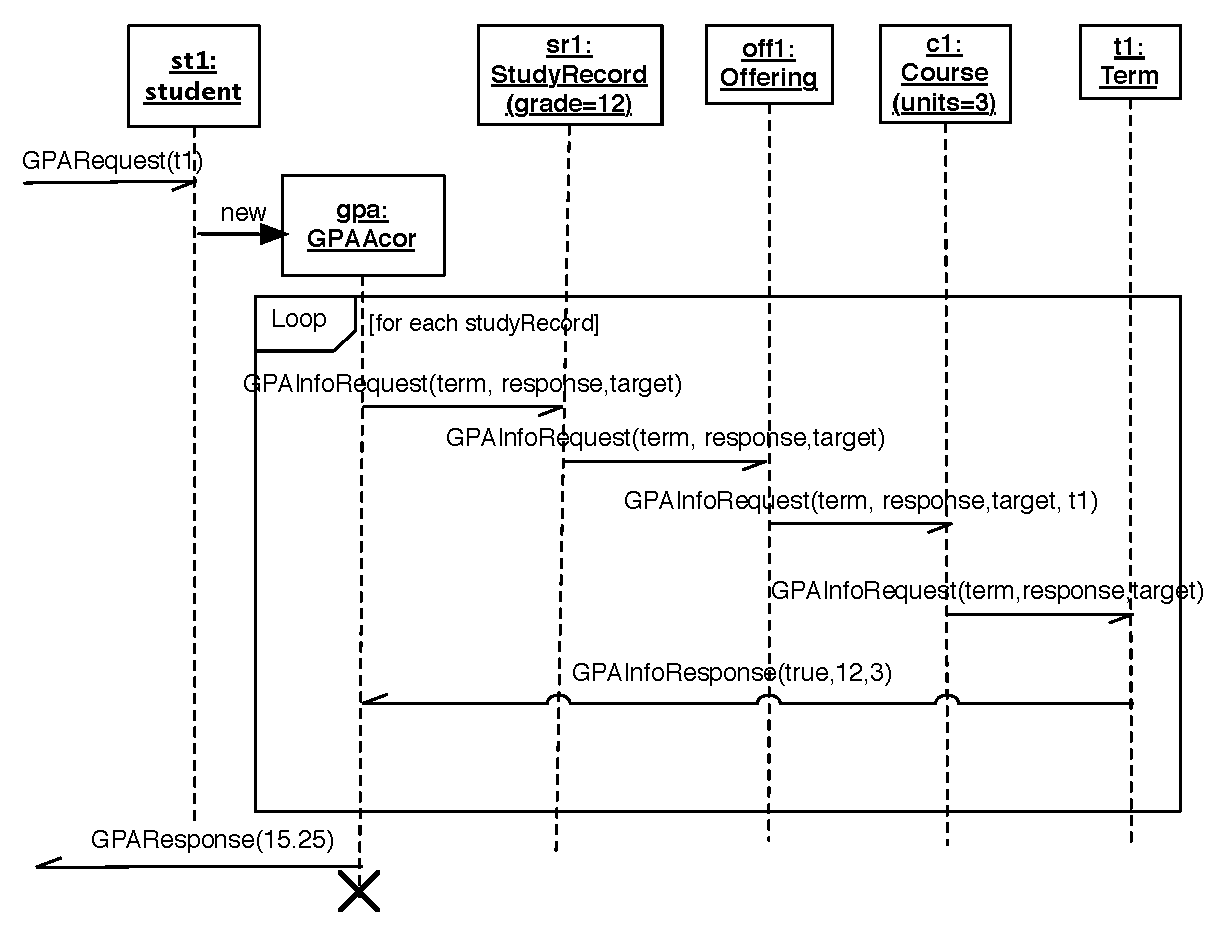
\includegraphics[width=16cm]{4-ProposedFramework/Figures/gpa_2_sequence.pdf}
    \end{center}
    \caption{\label{fig:gpa2_sequence} نمودار ترتیب برای رویکرد دوم محاسبه‌ی معدل }
\end{figure*}
\FloatBarrier
\begin{enumerate}
\item اکتور محاسبه‌ی معدل \lr{(GPAActor)}:\\
همان طور که قبلا توضیح داده شد، این اکتور برای انجام کل فعالیت‌های مربوط به یک درخواست معدل را انجام می‌دهد (در رویکرد اول این‌ کار توسط خود اکتور دانشجو انجام می‌شد).  این اکتور برای انجام وظیفه‌ی خود اولاً نیاز به برقراری ارتباط با اکتورهای سابقه دارد، و ثانیاً نیاز به دسترسی به مقصد پاسخ درخواست دارد تا بتواند نتیجه را برای آن ارسال کند. این موارد توسط اکتور دانشجو در اختیار اکتور محاسبه‌ی معدل قرار می‌گیرد. شبه کد \ref{fig:usecases:gpa:2:gpaActor} نحوه‌ی طراحی این اکتور را نشان می‌دهد. اکتور محاسبه‌ی معدل با شروع به کار پیغام‌های لازم برای سایر اکتور‌ها را ارسال می‌کند و با گرفتن هر پاسخ، متغیر‌های حالت خود را بروزرسانی می‌کند. پایان کار این اکتور زمانی مشخص می‌شود که به تعدادی که پیغام ارسال کرده پاسخ دریافت کند. این تعداد برابر با تعداد اکتورهای سابقه است. بنابراین پس از دریافت این تعداد پیغام، معدل محاسبه شده را برای مقصد نهایی ارسال می‌کند.

\codelisting[language=scala]{4-ProposedFramework/src/usecases/gpa/2/GPAActor.scala}{شبه‌کد طراحی اکتور محاسبه‌ی معدل در رویکرد ۲.}{fig:usecases:gpa:2:gpaActor} 

تغییر مهم اکتور دانشجو این است که با توجه به واگذاری عملیات محاسبه‌ی معدل به اکتوری دیگر، نیازی به نگهداری متغیرهای حالت که به این منظور ایجاد شده بودند، ندارد. شبه کد 
اکتور دانشجو در رویکرد جدید در شکل \ref{fig:usecases:gpa:2:student}  نشان داده شده است. مقایسه‌ی طراحی این اکتور در دو رویکرد نشان می‌دهد که با انجام این عمل، طراحی اکتور دانشجو بسیار ساده‌تر شده است.

\codelisting[language=scala]{4-ProposedFramework/src/usecases/gpa/2/Student.scala}{شبه‌کد طراحی اکتور دانشجو در رویکرد ۲.}{fig:usecases:gpa:2:student} 
\FloatBarrier

\end{enumerate}
%۱: نقش سابقه در این پیغام‌ها چیه؟ یکی اینکه نمره دست اونه و دیگه اینکه راهیه که به بقیه اطلاعات برسیم. اولی باعث می‌شه که حتما به دست اون برسه. ولی آیا اینکه جواب اول دست سابقه برسه بعد به دانشجو برسه الزامیه؟ با توجه به اینکه یک بار از زیر دستش رد می‌شه و دفعه‌ی دوم فقط relay می‌کنه.
%۲: یادآوری سوال ۲ بخش قبل. تاکید بر اینکه این بده چون ما همروندی رو پایین میاریم. آیا راهی برای این کار وجود نداره؟ یه اکتور درست می‌کنیم که فقط اینو ....
%۳: هیچ جا نمی‌شه مسیرو کوتاهتر کرد؟ زودتر جواب آخر رو فرستاد؟ منظور اینه که از domain بفهمیم. در این مورد اگر مربوط به ترم نباشه اصلا حساب نمی‌شه. پس اگه ترم ۱ سره بتونه جواب بده خیلی خوبه.
\subsubsection{مقایسه‌ی دو رویکرد}
در بخش‌های قبلی ۲ رویکرد متخلف برای طراحی اکتورها در ارتباط با مورد کاربرد محاسبه‌ی معدل معرفی شده و مراحل انجام طراحی در آنها شرح داده شد. علیرغم صحت عملکرد هر دو رویکرد، تفاوت‌های کیفی در طراحی به وسیله‌ی این دو رویکرد حائز اهمیت هستند. به همین دلیل در این بخش به مقایسه‌ی این دو رویکرد می‌پردازیم.\\
رویکرد دوم دو تغییر عمده نسبت به رویکرد اول دارد:
\begin{enumerate}
\item قرار دادن مقصد نهایی درخواست در داخل پیغام:\\
در رویکرد اول هر اکتوری که پیغامی را به عنوان درخواست از یک اکتور دیگر دریافت می‌کند، وظیفه‌ی پاسخ به آن را نیز به عهده دارد. در صورتی که برای پاسخ به درخواست نیاز به برقراری ارتباط با اکتورهای دیگر وجود داشته باشد،‌این اکتور اقدام به ارسال پیغام‌های مرتبط به سایر اکتورها می‌کند و در نهایت با جمع‌آوری پاسخ‌ها، درخواست اصلی را پاسخ می‌دهد. با اینکه این رویکرد از دیدگاه طراحی شیءگرا به روش ترتیبی،‌ رویکردی متداول و حتی اجباری است\footnote{در طراحی شیءگرای ترتیبی، مکانیزم کنترل برنامه فراخوانی متد است. با هر فراخوانی متد، منطق پیاده شده در متد اجرا می‌شود و پس از بازگشت از متد، اجبارا کنترل برنامه به همان قسمتی که متد فراخوانی شده بود برمی‌گردد.}، در مدل تبادل پیغام این امکان وجود دارد که پاسخ درخواست را اکتوری غیر از دریافت کننده‌ی درخواست ارسال کند. لازم به ذکر است که در مدل اکتور هیچ فرضی در مورد مشخصات فرستنده‌ی پیغام صورت نمی‌گیرد. بنابراین یک اکتور می‌تواند به جای اینکه پس از ارسال پیغام‌های مربوط به یک درخواست، منتظر دریافت جواب برای فرستادن به درخواست کننده بماند،‌ آدرس (نام) مقصد نهایی را در داخل پیغام برای اکتور ها ارسال کند تا در صورت لزوم از آن برای فرستادن نتیجه استفاده کنند. رویکرد دوم در واقع از این امتیاز استفاده کرده و به این روش از تعدادی از تبادلات پیغام که صرفاً به دلیل ذکر شده صورت می‌گیرند، جلوگیری می‌کند. با این کار نیازی به برگشت پیغام در همان مسیری که طی شده وجود نخواهد داشت و در هر لحظه که اطلاعات لازم برای تکمیل پاسخ تأمین شود، پاسخ به مقصد ارسال خواهد شد.
\item واگذار کردن پردازش‌های مربوط به یک درخواست به یک اکتور موقت:\\
 در رویکرد اول اکتور دانشجو، پس از ارسال پیغام‌های لازم و دریافت جواب، تمام محاسبات لازم برای تعیین معدل را انجام ‌می‌داد. در اثر استفاده از این رویکرد، اولاً دانشجو باید تعدادی پیغام برای تهیه‌ی اطلاعات لازم جهت محاسبه‌ی معدل به سایر اکتورها ارسال کرده و منتظر جواب بماند، ثانیاً برای محاسبه‌ی معدل اطلاعات موقتی را به عنوان متغیر حالت در خود نگهداری کند. مقدار این متغیر‌ها فقط در زمانی که یک درخواست مشخص در حال پردازش است معتبر است به همین دلیل در صورت شروع به پردازش درخواست‌های دیگر قبل از اتمام عملیات مربوط به درخواست قبلی امکان‌پذیر نمی‌باشد. در نتیجه میزان همروندی در درخواست‌های مشابه پایین می‌آید. از طرف دیگر در صورتی که قرار باشد، اکتور انواع متعددی از درخواست‌هایی را که این خاصیت را دارند پردازش کند، مدیریت پیچیدگی حاصل از اطلاعات حالت مربوط به درخواست‌های مختلف نیز کار آسانی نخواهد بود و منجر به پیچیدگی زیاد  و تغییرپذیری کمتر کلاس خواهد شد. به همین دلایل در رویکرد دوم سیاست جدید اتخاذ شد و آن سپردن کل فعالیت‌های محاسبه‌ی معدل به یک اکتور جدید است. با این کار دو نتیجه‌ی مطلوب حاصل می‌شود. اولاً پیچیدگی‌های مربوط به اجرای یک درخواست به اکتور دیگری منتقل می‌شود که صرفاً برای پاسخ به درخواست مورد نظر طراحی شده است. ثانیا با توجه به اینکه هر نمونه از اکتور جدید صرفاً محدود به یک درخواست بوده و پس از پاسخ به‌ آن به فعالیت خاتمه می‌دهد، امکان پاسخ به درخواست‌های همروند به درخواست‌ها هم به وجود می‌آید.
\end{enumerate}
لازم به ذکر است که هدف از معرفی این دو رویکرد در طراحی منطق مربوط به محاسبه‌ی معدل صرفاً تأکید بر تفاوت‌های آنها و حفظ وضوح روش طراحی دارد. طبیعتاً علیرغم صحت رویکرد اول، در ادامه‌ی طراحی از سیاست‌های ذکر شده در رویکرد دوم استفاده خواهد شد
\subsection{مورد کاربرد اخذ درس}
در بخش قبل مراحل طراحی مورد کاربرد محاسبه‌ی معدل با استفاده از دو رویکرد مختلف توضیح داده شد. در این بخش مراحل طراحی مورد کاربرد اخذ درس با توجه به تجربیات حاصل از بخش قبل ارائه می‌گردد. \\
توصیف مورد کاربرد اخذ درس در جدول \ref{table:uc_takecoure} ارائه شد. دانشجو در زمان انتخاب واحد یکی از ارائه‌\LTRfootnote{Offering}های موجود ترم را انتخاب می‌کند. سیستم شرایط لازم برای اخذ این ارائه را بررسی می‌کند. در صورتی که دانشجو مجاز به انتخاب این ارائه باشد، یک سابقه از ارائه‌ی مورد نظر را برای دانشجو ذخیره می‌کند. در صورتی که هر کدام از شرایط لازم برای اخذ محقق نشده باشد سیستم یک پیغام خطا برای کاربر نمایش می‌دهد.
همانند مورد کاربرد قبل،‌ این مورد کاربرد هم با دریافت یک پیغام توسط اکتور دانشجو آغاز می‌شود. تنها اطلاعاتی که در این پیغام باید موجود باشد ارائه‌ی انتخاب شده برای اخذ است. بنابراین فرمت پیغام درخواست اخذ درس به شکل زیر خواهد بود:
\begin{latin}
TakeCourseRequest(offering: Offering)
\end{latin}
پاسخ این درخواست نیز باید حاوی نتیجه‌ی عملیات و نیز احتمالاً یک پیغام برای کاربر خواهد بود. بنابراین پیغام پاسخ اخذ درس به فرمت زیر خواهد بود:
\begin{latin}
TakeCourseResponse(result: Boolean, comment: String)
\end{latin}
مطابق توضیحاتی که در طراحی مورد کاربرد محاسبه‌ی معدل داده ‌شد، اکتور دانشجو در مواجهه با پیغام درخواست اخذ دو راهکار کلی پیش رو دارد. راهکار اول این است که منطق مورد نیاز برای پردازش اخذ درس را خودش پیاده‌سازی کند (مانند رویکرد اول در طراحی مورد کاربرد محاسبه‌ی معدل) و راهکار دوم این است که به یک اکتور دیگر وکالت این محاسبات را بسپارد. همان‌طور که در بخش قبل ذکر شد،‌ تصمیم به سپردن محاسبات به کاربرد دیگر به دو انگیزه‌ی مختلف صورت می‌گیرد. انگیزه‌ی اول جلوگیری از پیجیده و بزرگ شدن یک اکتور در اثر پردازش پیغام‌های مختلف و انگیزه‌ی دوم ایجاد امکان همروندی در پردازش پیغام‌های مشابه.\\
در این مورد کاربرد هر دو انگیزه برای سپردن محاسبات به یک اکتور دیگر معتبر می‌باشند: اکتور دانشجو در مدل دامنه‌ی معرفی شده، مسئولیتِ دریافت اکثر درخواست‌های کاربران را به عهده دارد (به دلیل اینکه کاربر اصلی این سیستم دانشجو است)، درخواست‌های مختلفی را دریافت خواهد کرد. به همین دلیل در صورتی که  پردازش تمام این پیغام‌ها را بر عهده بگیرد، اندازه و پیچیدگی آن زیاد شده و در نتیجه تغییرپذیری آن تنزّل خواهد کرد (انگیزه‌ی اول). علاوه بر این، اکتور دانشجو برای پردازش هر درخواست اخذ درس، باید شروط مختلفی را بررسی کند و برای این کار با اکتورهای دیگر به دفعات تبادل پیغام انجام خواهد داد و برای حفظ نتایج میانی تبادلات پیغام تا پایان پردازش درخواست، مجبور به استفاده از متغیرهای حالت اکتور (فیلدهای داده‌ی محلی) خواهد بود (مشابه متغیرهایی که در محاسبه‌ی معدل استفاده شد). در نتیجه پردازش همروند درخواست‌های اخذ درس بسیار پیچیده و یا نشدنی خواهد بود. بنابراین در این مورد، ایجاد همروندی در پردازش درخواست‌ها نیز انگیزه‌ی معتبری برای سپردن محاسبات به یک اکتور دیگر است (انگیزه‌ی دوم). \\
\subsubsection{ اکتور اخذ درس}
\label{section:takeCourse}
با توجه به توضیحات ذکر شده اکتور دانشجو با گرفتن درخواست اخذ درس، کلیه‌ی محاسبات لازم و ارسال پاسخ را به اکتور اخذ درس منتقل می‌کند. وظیفه‌ی اکتور اخذ درس بررسی شرایط دانشجو برای اخذ درس و ارسال پاسخ درخواست است. طبق توصیف مورد کاربرد اخذ درس (جدول \ref{table:uc_takecoure})، شروطی که باید قبل از قبول اخذ درس بررسی شوند عبارتند از:
\begin{enumerate}
\item دانشجو در ترم‌های قبل درس مربوط به ارائه‌ی انتخاب شده را  نگذرانده باشد.
\item دانشجو در ترم‌ جاری این درس را اخذ نکرده باشد.
\item دانشجو تمام پیش‌نیاز‌های این درس را با موفقیت گذرانده باشد.
\item تعداد واحد‌های اخذ شده توسط دانشجو در این ترم پس از اخذ این درس بیشتر از ۲۰ نشود.
\end{enumerate}
در این مرحله، اکتور اخذ درس باید برای هریک از شروط ذکر شده، اولاً قالب پیغام مناسب را طراحی کند، ثانیاً مقصد پیغام را مشخص کند (تشخیص اکتور مسئول). این دو مورد باید برای هریک از چهار شرط فوق بررسی شوند. در ادامه بررسی این موارد برای شرط اول به صورت مبسوط بررسی می‌شود و برای سایر شروط با توجه به شباهت به شرط اول صرفاً نتیجه‌ی بررسی ارائه می‌گردد:
\begin{itemize}
\item شرط ۱:\\
 این شرط باید تعیین کند که دانشجو قبلاً سابقه‌ای از گذراندن این درس را دارد یا خیر. قبل از انتخاب قالب پیغام، بحثی در مورد پذیرنده‌ی پیغام (اکتور مسئول) می‌کنیم. گزینه‌های موجود برای اکتور مسئول بررسی شرط گذراندن درس باشد اینها هستند:
 \begin{enumerate}
 \item خود اکتور اخذ درس:\\
  انتخاب اول در واقع به این معنی است که اکتور اخذ درس به جای اینکه درخواستی برای بررسی گذرانده شدن درس ارسال کند،‌ خود این بررسی را به عهده بگیرد. البته این به این معنی نیست که برای انجام این بررسی هیچ پیغامی به اکتورهای دیگر ارسال نکند، بلکه به این معنی است که وظیفه‌ی پیاده‌سازی منطق لازم برای رسیدن به پاسخ این پرسش (آیا این دانشجو قبلاً این درس را گذرانده است؟) بر عهده‌ی اکتور اخذ درس باشد. این حالت به دو دلیل مناسب نیست: اولاً در این حالت اکتور اخذ درس به صورت ابتدا به ساکن (بدون دریافت درخواستی برای این کار) اقدام به پیاده‌سازی یک منطق کرده است. در نتیجه این پیاده‌سازی به جز این اکتور برای اکتور دیگری قابل استفاده‌ی مجدد نیست.
 \footnote{  البته یک راهکار ممکن برای برطرف کردن این مشکل این است که به اکتور اخذ درس، قابلیت دریافت پیغامی از نوع بررسی شرط مذکور اضافه شود و این اکتور برای بررسی این شرط، یک پیغام به خودش بفرستد تا به این صورت قابلیت استفاده‌ی مجدد داشته باشد. اما ایراد این رویکرد این است که از نظر منطقی اضافه کردن این رفتار به اکتوری که صرفاً وظیفه‌ی پاسخ به یک درخواست اخذ درس را دارد، از نظر تقسیم مسئولیت عمل درستی نیست.}
  ثانیاً با توجه به اینکه این اکتور شروط متعددی را بررسی می‌کند، پیاده کردن منطق بررسی این شروط خوانایی کلاس را کاهش می‌دهد. 
 
  البته یک راهکار ممکن برای برطرف کردن این مشکل این است که به اکتور اخذ درس، قابلیت دریافت پیغامی از نوع بررسی شرط مذکور اضافه شود و این اکتور برای بررسی این شرط، یک پیغام به خودش بفرستد تا به این صورت قابلیت استفاده‌ی مجدد داشته باشد. اما ایراد این رویکرد این است که از نظر منطقی اضافه کردن این رفتار به اکتوری که صرفاً وظیفه‌ی پاسخ به یک درخواست اخذ درس را دارد، از نظر تقسیم مسئولیت عمل درستی نیست. 
 \item اکتور جدیدی که به این منظور تولید می‌شود:\\
 این رویکرد ایرادهای شمرده شده برای انتخاب اول را ندارد. اما با فرض این که درخواست بررسی گذرانده شدن درس یک درخواست قابل استفاده‌ی مجدد در منطق دامنه‌ی سیستم باشد، با این رویکرد در هر قسمتی از برنامه که نیاز به بررسی این درخواست وجود داشته باشد، باید اکتوری به این منظور ایجاد شود و اطلاعات لازم به آن داده شود و سپس درخواست برای آن ارسال شود. از نظر طراحی شیءگرا، تکرار این عملیات در هر بار نیاز به این درخواست پدیده‌ی مطلوبی نمی‌باشد.
 \item اکتور دانشجو:\\
 انتخاب اکتور دانشجو برای ارسال درخواست بررسی گذرانده شدن درس علاوه بر اینکه ایرادهای مطرح شده در گزینه‌ی اول را ندارد، مشکل تکرار عملیات (گزینه‌ی دوم) را نیز ندارد. در این حالت، هر اکتوری که نیاز به بررسی درخواست گذرانده شدن درس را داشته باشد، پیغام مربوطه را برای اکتور دانشجو ارسال می‌کند و تنها جایی که عملیات ایجاد اکتور جدید برای پردازش این درخواست انجام می‌شود اکتور دانشجو است. از نظر منطق دامنه نیز بررسی گذرانده شدن درس توسط اکتور دانشجو انتخاب مطلوبی به نظر می‌رسد.
 \end{enumerate}
 با توجه به استدلال فوق، اکتور اخذ درس، اکتور دانشجو را به عنوان مسئول بررسی گذرانده شدن درس انتخاب می‌کند.\\
 با انتخاب مقصد پیغام درخواست بررسی گذرانده شدن درس، طراحی قالب پیغام آن به آسانی انجام می‌شود. با توجه به اینکه این پیغام به مقصد اکتور دانشجو ارسال می‌شود، تنها داده‌ای که لازم است در آن قرار داده شود درس مربوطه است. بنابراین قالب پیغام درخواست به صورت زیر می‌باشد:
 \begin{latin}
 PassedRequest(course:Course)
 \end{latin}
 پیغام پاسخ کافی‌ است که اطلاع دهد که درس مورد نظر گذرانده شده است یا خیر. بنابراین قالب پیغام پاسخ به صورت زیر می‌باشد:
 \begin{latin}
PassedResponse(result:Boolean)
 \end{latin}
% با توجه به توضیحات داده‌ شده، طراحی اکتور اخذ درس تا این مرحله از طراحی به صورت شبه‌کد شکل بلاه خواهد بود.

\item شرط ۲:\\
 این شرط باید تعیین کند که دانشجو قبلاً در همین ترم این درس را اخذ کرده است یا خیر. با استدلال مشابه شرط ۱ به این نتیجه می‌رسیم که مقصد پیغام درخواست بررسی اخذ تکراری اکتور دانشجو است و قالب پیغام‌های درخواست و پاسخ برای این شرط به صورت زیر می‌باشد:
 \begin{latin}
 TakenRequest(course:Course)
 TakenResponse(result:Boolean)
 \end{latin}

\item شرط ۳:\\
 این شرط باید تعیین کند که دانشجو تمام پیش‌نیازهای درس را با موفقیت گذرانده است یا خیر. با استدلال مشابه شرط ۱ به این نتیجه می‌رسیم که مقصد پیغام درخواست بررسی اخذ تکراری اکتور دانشجو است و قالب پیغام‌های درخواست و پاسخ برای این شرط به صورت زیر می‌باشد:
 \begin{latin}
 PassedPresRequest(course:Course)
 PassedPresResponse(result:Boolean)
 \end{latin}
 
\item شرط ۴:\\
 این شرط کنترل می‌کند که با اخذ این درس آیا تعداد واحدهای دانشجو در ترم جاری بیشتر از ۲۰ می‌شود یا خیر. گذراندن بیش از تعدادی واحد به احتمال زیاد در چنین سیستمی به جز در بررسی شرایط کاربرد دیگری ندارد (بر خلاف موردی مثل بررسی گذرانده شدن درس که در موارد متعددی می‌تواند کاربرد داشته باشد) به همین دلیل پیغام مربوط به این مورد بهتر است به جای دانشجو به اکتور دیگری که مختص این کاربرد طراحی می‌شود سپرده شود. گیرنده‌ی پیغام مربوط به این شرط اکتور تأیید تعداد واحد (UnitsValidatorActor)  خواهد بود. با توجه به این که اکتور مذکور نیاز به دسترسی به سوابق دانشجو و نیز تعداد واحد درس انتخاب شده دارد، در هنگام ایجاد این اکتور، باید فیلد‌های دانشجو و درس را در اختیار اکتور قرار دهیم. به این ترتیب، اکتور تأیید تعداد واحد به محض ایجاد می‌تواند کار خود را شروع کند و  اکتور اخذ درس نیازی به ارسال پیغام به آن ندارد. با توجه به این توضیحات پیغام‌ پاسخ برای این شرط به صورت زیر می‌باشد:
 \begin{latin}
  UnitsValidationResponse(result:Boolean)
 \end{latin}
\end{itemize}
در این مرحله باید تعیین کنیم که اکتور بررسی اخذ درس با دریافت پاسخ هر پیغام چه عملی را باید انجام دهد:\\
هر یک از پاسخ‌هایی که اکتور بررسی اخذ درس دریافت می‌کند در واقع نتیجه‌ی بررسی یکی از شروط لازم برای اخذ درس است. برای موافقت با اخذ درس توسط دانشجو، تمام شروط باید بررسی شوند. بنابراین پاسخ موافقت با اخذ درس فقط زمانی می‌تواند ارسال شود که تمام پاسخ‌ها دریافت شوند. برای اینکه اکتور اخذ درس از اتمام دریافت دروس مطلع شود لازم است که متغیری به منظور نگه‌داری تعداد پاسخ‌هایی که باید دریافت شود ایجاد شده بروزرسانی شود. با این کار اکتور اخذ درس می‌داند که چه زمانی کار به اتمام رسیده است. اما در این مورد کاربرد، در همه‌ی حالت‌ها لازم نیست اکتور منتظر تمام پاسخ‌ها بماند. دلیل این امر این است که در صورتی که هر یک از شروط اخذ درس نقض شود، نیازی به بررسی سایر شروط نیست. مثلاً اگر دانشجو قبلاً درس را گذرانده باشد نیازی به دریافت سایر پاسخ‌ها وجود ندارد و می‌توانیم پاسخ درخواست را ارسال کنیم (خطای گذرانده شدن درس). بنابراین در این مورد کاربرد با گرفتن هر پاسخ به این ترتیب عمل می‌کنیم که اگر شرط برقرار باشد، مقدار متغیر تعداد پاسخ‌های دریافت شده را یکی زیاد می‌کنیم، اگر مقدار جدید برابر با تعداد پاسخ مورد انتظار بود (این یعنی تمام پاسخ‌ها دریافت شده‌اند)، پاسخ نهایی درخواست را ارسال می‌کنیم. و اگر شرط نقض شده باشد پاسخ درخواست را که عدم موفقیت اخذ به دلیل نقض شرایط است ارسال می‌کنیم.
نمودار شکل \ref{fig:take_course_sequence_1} تصمیمات اتخاذ شده تا این مرحله از طراحی را به صورت شماتیک نشان می‌دهد. در این نمودار حالتی بررسی شده که تمام شرایط اخذ درس برقرار شده و اخذ با موفقیت انجام می‌شود. حالت دیگری که یکی از شروط (تعداد واحد) برقرار نشده است در شکل \ref{fig:take_course_sequence_2} نشان داده شده است. در این حالت با توجه به اینکه یکی از پاسخ‌ها نشان‌دهنده‌ی این است که یکی از شروط برقرار نشده،‌ به محض دریافت این پیغام، اکتور اخذ درس نتیجه‌ی درخواست را ارسال می‌کند و به کار خود پایان می‌دهد. طبیعتا پیغام‌های دیگری که برای این اکتور ارسال شده‌اند پردازش نخواهند شد.
لازم به تأکید است که در هر دو شکل ترتیب پیغام‌ها فقط نشان دهنده‌ی یک حالت فرضی هستند. در عمل در هر بار اجرای برنامه، ترتیب گرفتن پاسخ‌ها ممکن است عوض شود.

\begin{figure*}
    \begin{center}
	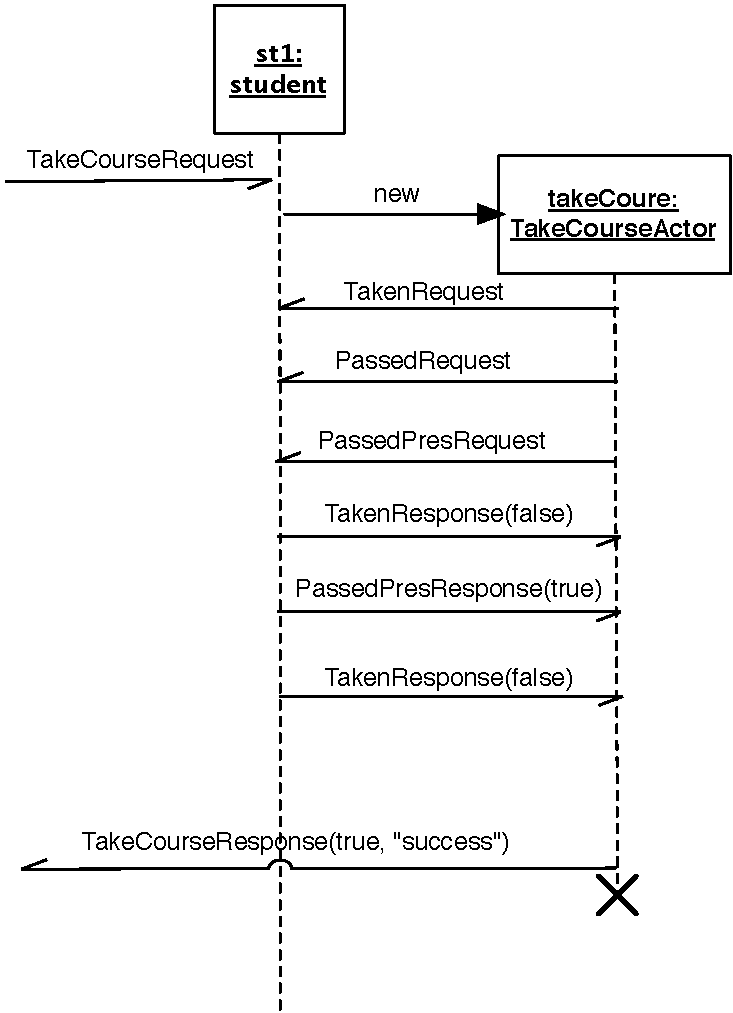
\includegraphics[width=14cm]{4-ProposedFramework/Figures/take_course_seq1.pdf}
    \end{center}
    \caption{\label{fig:take_course_sequence_1} نمودار ترتیب تبادل پیغام‌ برای اخذ درس- حالتی که تمام شروط برای اخذ برقرار است }
\end{figure*}
%\FloatBarrier

\begin{figure*}
    \begin{center}
	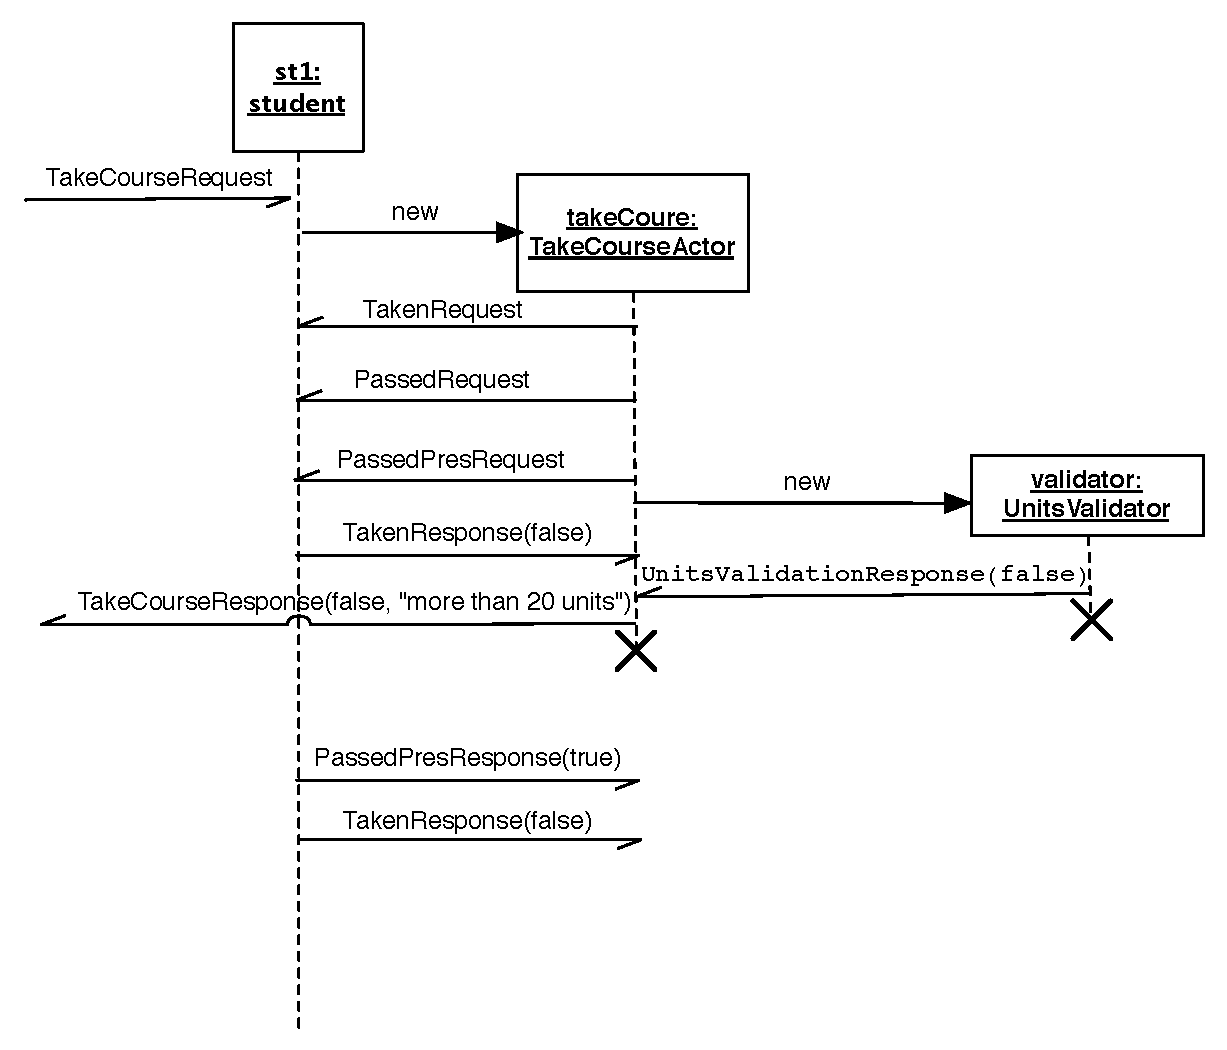
\includegraphics[width=14cm]{4-ProposedFramework/Figures/take_course_seq2.pdf}
    \end{center}
    \caption{\label{fig:take_course_sequence_2} نمودار ترتیب تبادل پیغام‌ برای اخذ درس- حالتی که یکی از شروط برقرار نیست }
\end{figure*}
%\FloatBarrier


 در این مرحله، طراحی اکتور اخذ درس به پایان رسیده است. شبه‌کد \ref{fig:usecases:take_course:take_course} ساختار کلاس اکتور اخذ درس را نشان می‌دهد.
 \codelisting[language=scala]{4-ProposedFramework/src/usecases/take_course/TakeCourseActor.scala}{شبه‌کد طراحی اکتور اخذ دانشجو.}{fig:usecases:take_course:take_course} 
%\FloatBarrier
  در ادامه باید تغییرات سایر اکتورها در اثر دریافت پیغام‌های ارسال شده از اکتور اخذ درس اعمال شود و نیز اکتور جدیدی که ایجاد شده (اکتور تایید تعداد واحد) نیز طراحی گردد.
%   برای رعایت اختصار و اجتناب از طرح نکات تکراری، جزئیات طراحی بررسی شرط گذرانده شدن درس‌ ارائه می‌گردد.
\subsubsection{بررسی گذرانده شدن درس}
\label{subsection:passCourse}
  برای بررسی گذرانده شدن درس، اکتور اخذ درس یک پیغام CoursePassRequest به اکتور دانشجو ارسال می‌کند. اکتور دانشجو بررسی این شرط را به اکتور جدید گذراندن درس\LTRfootnote{CoursePassActor} می‌سپارد. این اکتور برای بررسی گذرانده شدن درس، نیاز به برقراری ارتباط با اکتورهای سابقه\LTRfootnote{StudyRecord} دارد. بنابراین اکتور دانشجو لیست سابقه‌ی دانشجو و نیز درسی که باید گذرانده شدن آن بررسی شود را در اختیار اکتور بررسی گذراندن درس قرار می‌دهد. اکتور گذراندن درس از تمام اکتورهای سابقه سؤال می‌کند که آیا سابقه‌ی مربوطه یک گذراندن موفق از درس مذکور است یا خیر. این کار با ارسال یک پیغام با قالب زیر صورت می‌پذیرد:
  \begin{latin}
  AreYouPassCourseRequest(course)
  \end{latin}
هر اکتور سابقه‌ با دریافت این پیغام باید اولاً بررسی کند که آیا سابقه‌ای مربوط به درس مذکور است یا خیر، و ثانیاً نمره‌ی سابقه نمره‌ی قبولی است یا خیر. در اینجا با توجه به اینکه نمره‌ی مربوطه در اختیار خود اکتور سابقه است، بررسی آن ساده‌تر است. در صورتی که نمره کمتر از ۱۰ باشد، این اکتور بلافاصله پاسخ پیغام (منفی) را می‌دهد، در غیر این صورت برای بررسی این که این سابقه مربوط به درس مذکور است یا خیر، یک پیغام برای اکتور ارائه ارسال می‌کند. اکتور ارائه با گرفتن این پیغام آن را برای اکتور درس ارسال می‌کند تا این اکتور بررسی کند که آیا با درسی که در قالب پیغام دریافت کرده برابر است یا خیر. این اکتور پاسخ نهایی را مستقیماً برای اکتور بررسی گذرانده شدن درس ارسال می‌کند.  
\begin{figure}
    \begin{center}
	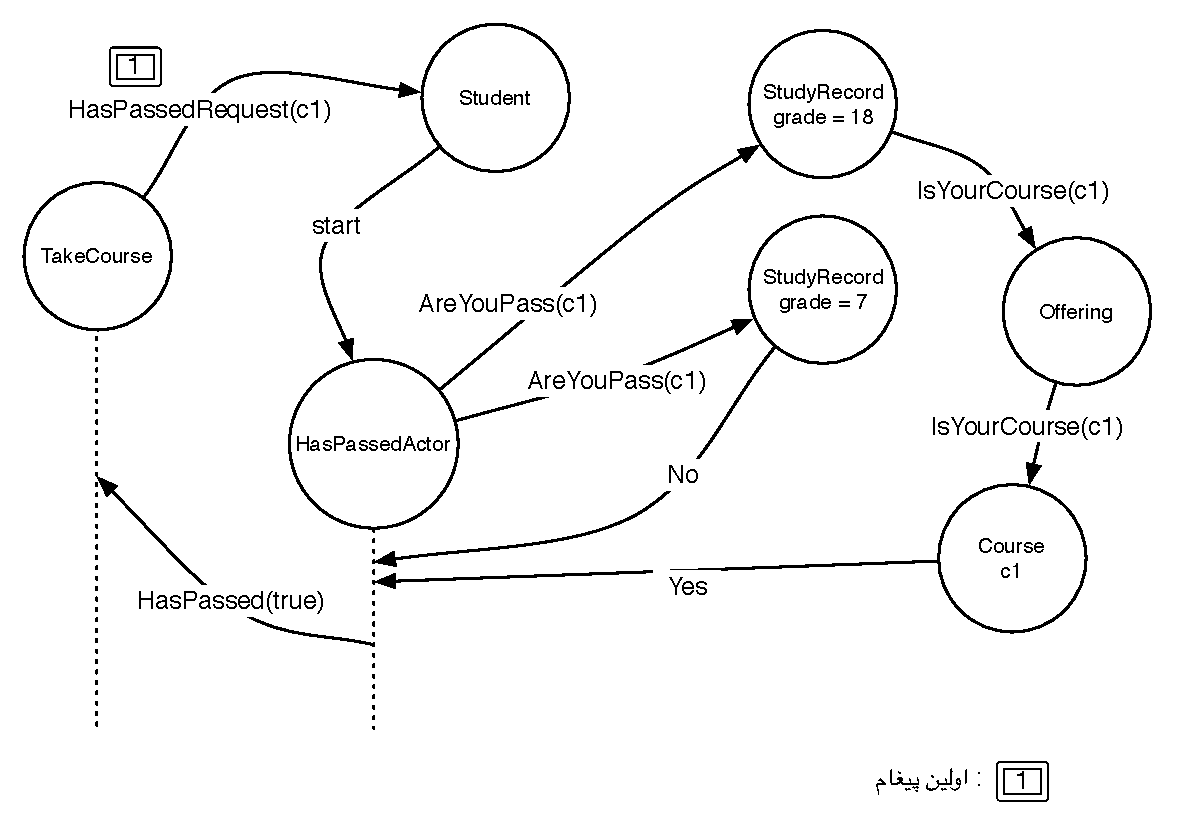
\includegraphics[width=14cm]{4-ProposedFramework/Figures/HasPassed.pdf}
    \end{center}
    \caption{\label{fig:take_course_haspassed}نمایش شماتیک تبادل پیغام بین اکتورهای مختلف برای بررسی گذرانده شدن یک درس }
\end{figure}

شکل \ref{fig:take_course_haspassed} تبادل پیغام‌های مربوط به بررسی گذرانده شدن درس را به صورت شماتیک نشان می‌دهد. در این شکل خط عمودی در حالتی به کار رفته‌ است که یک اکتور در زمان‌های مختلف پیغام دریافت کرده باشد. در مثال بررسی شده در شکل، اکتور اخذ درس یک درخواست بررسی گذرانده شدن درس (درس c1 ( را برای اکتور دانشجو ارسال می‌کند. اکتور دانشجو یک اکتور بررسی گذرانده شدن درس (HasPassedActor) ایجاد می‌کند و کار بررسی را به آن واگذار می‌کند. این اکتور پیغام‌های مناسب را برای دو اکتور سابقه‌ی دانشجو ارسال می‌کند. یکی از اکتورهای سابقه به این دلیل که نمره‌ی کمتر از ۱۰ (۷) دارد، بلافاصله پاسخ را برای اکتور مقصد ارسال می‌کند. اکتور سابقه‌ی دیگر با توجه به اینکه نمره‌ی قبولی دارد،‌ برای اطمینان از اینکه مربوط به همان درسی است که گذرانده شدن آن بررسی می‌شود، یک پیغام به اکتور ارائه ارسال می‌کند. اکتور ارائه پیغام را به درس منتقل می‌کند و اکتور درس با مقایسه‌ی درس موجود در پیغام با خودش، جواب را برای مقصد می‌فرستد.
\FloatBarrier
\subsubsection{بررسی گذرانده شدن پیش‌نیازهای درس}
اکتور دانشجو با دریافت پیغام بررسی گذرانده شدن پیش‌نیازهای درس، محاسبات مربوطه را به اکتوری که به این منظور طراحی شده ارسال می‌کند. با توجه به اینکه پیش‌نیازهای هر درس نیز خود از نوع درس هستند، در طراحی این بخش می‌توان از اکتور بررسی گذرانده شدن درس استفاده کرد. بنابراین اکتور مذکور به ازای هر کدام از پیش‌نیازهای درس، یک پیغام بررسی گذرانده شدن درس به دانشجو ارسال می‌کند. با دریافت هر پاسخ اگر مشخص شود که درسی از میان پیش‌نیازها گذرانده نشده است، بلافاصله پاسخ درخواست به مقصد (اکتور اخذ درس) ارسال می‌شود. در غیر این صورت پس از گرفتن تمام پاسخ‌ها، یک پیغام به اکتور اخذ درس ارسال می‌کند و به وسیله‌ی آن اعلام می‌کند که تمام پیش‌نیازها گذرانده شده است.
\begin{figure}
    \begin{center}
	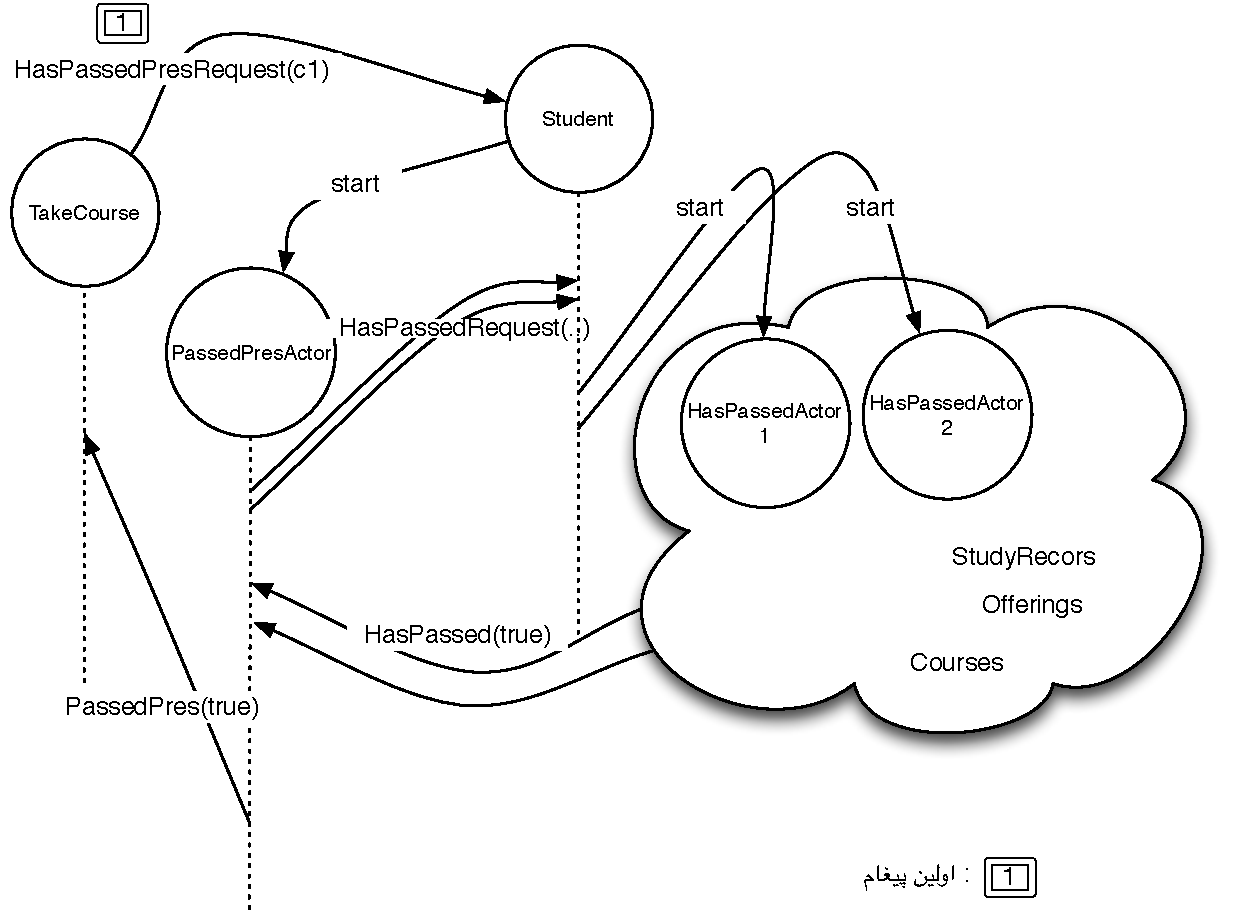
\includegraphics[width=14cm]{4-ProposedFramework/Figures/Prerequisites.pdf}
    \end{center}
    \caption{\label{fig:take_course_pres}نمایش شماتیک تبادل پیغام بین اکتورهای مختلف برای بررسی گذرانده شدن پیشنیازها‌ی یک درس }
\end{figure}
شکل \ref{fig:take_course_pres} ارتباط اکتورها برای بررسی گذرانده شدن درس نشان می‌دهد. در این شکل، ابتدا اکتور اخذ درس پیغام بررسی گذرانده شدن درس c1 را به اکتور دانشجو ارسال می‌کند. اکتور دانشجو بررسی بررسی این مورد را به اکتور بررسی پیش‌نیاز\LTRfootnote{PassPresActor} واگذار می‌کند. این اکتور به ازای هر کدام از پیشنیاز‌های  درس، یک پیغام بررسی گذرانده شدن درس برای خود دانشجو ارسال می‌کند. طراحی مورد بررسی گذراندن درس در بخش \ref{subsection:passCourse} توضیح داده شد. در این شکل برای جلوگیری از پیچیدگی طراحی، از نمایش نحوه‌ی بررسی گذرانده شدن درس صرف نظر شده است و اکتورها و پیغام‌های مربوط به آن به صورت شکل ابر نمایش داده شده است.

\FloatBarrier
\subsubsection{بررسی عدم اخذ مجدد درس}
همان‌طور که در بخش \ref{section:takeCourse} توضیح داده شد، اکتور اخذ درس یک پیغام برای بررسی عدم اخذ مجدد درس برای اکتور دانشجو ارسال می‌کند. اکتور دانشجو مطابق حالت‌های قبل بررسی این مورد را به اکتور بررسی اخذ درس\LTRfootnote{CourseTakenCheckActor} واگذار می‌کند. بررسی  اخذ شدن درس کاملاً مشابه بررسی گذرانده شدن درس است. در بررسی گذرانده شدن درس، اکتور سابقه نمره را بررسی می‌کند، در صورتی که نمره قبولی نباشد جواب را ارسال می‌کند و در صورتی که نمره قبولی باشد برای بررسی اینکه درس مربوط به سابقه همان درس مورد سؤال است یا خیر، با اکتور ارائه تبادل پیغام انجام می‌دهد. در بررسی عدم اخذ مجدد درس، از هر اکتور سابقه سؤال می‌شود که آیا سابقه مربوط به ترم جاری است یا خیر. برای اینکه  یک سابقه مربوط به ترم جاری باشد، کافی است نمره‌ای برای آن اعلام ثبت نشده باشد. بنابراین اکتور سابقه بررسی می‌کند که نمره‌ای برایش ثبت شده یا خیر اگر مقدار فیلد نمره null باشد یعنی مربوط به ترم جاری است و برای بررسی اینکه مربوط به همان درس مورد سؤال است مانند حالت بررسی گذرانده شدن درس، یک پیغام به ارائه ارسال می‌کند. در غیر این صورت حتماً جواب منفی است و بلافاصله یک پیغام برای اکتور بررسی عدم اخذ مجدد ارسال می‌شود. شکل  \ref{fig:take_course_taken} تبادل پیغام بین اکتورها برای بررسی این شرط را نشان می‌دهد. همان‌طور که مشاهده می‌شود این شکل بسیار شبیه به شکل \ref{fig:take_course_haspassed} است که بررسی گذرانده شدن درس را نشان می‌دهد.

\begin{figure}
    \begin{center}
	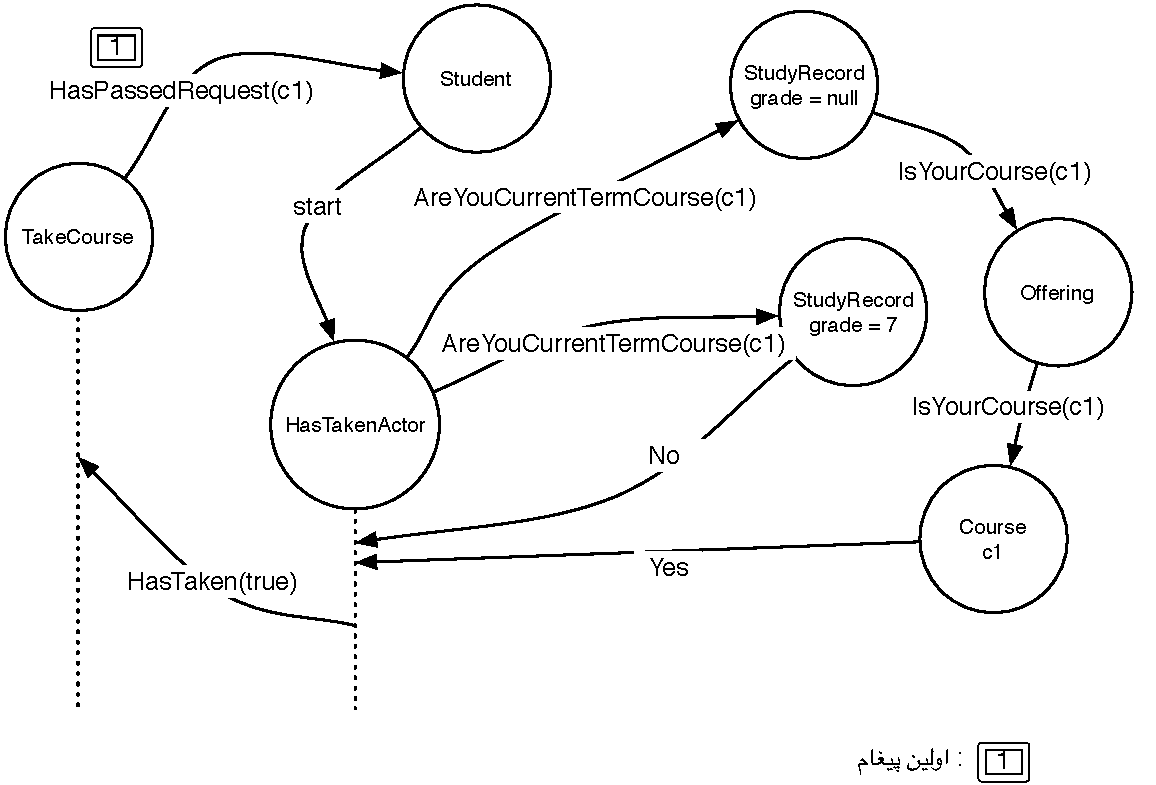
\includegraphics[width=14cm]{4-ProposedFramework/Figures/HasTaken.pdf}
    \end{center}
    \caption{\label{fig:take_course_taken}نمایش شماتیک تبادل پیغام بین اکتورهای مختلف برای بررسی عدم اخذ مجدد درس }
\end{figure}





\FloatBarrier
\subsubsection{بررسی عدم اخذ بیش از ۲۰ واحد}
در بخش طراحی اکتور اخذ درس (بخش \ref{section:takeCourse}) دیدیم که اکتور اخذ درس برای بررسی این شرط که تعداد واحدهای اخذ شده بیشتر از ۲۰ نشود، یک اکتور به این منظور ایجاد می‌کند. این اکتور با بررسی این شرط نتیجه را به صورت پیغام UnitsValidationResponse برای اکتور اخذ درس ارسال می‌کند. طراحی این کارکرد به این صورت است که اکتور مورد نظر از تمام سابقه‌های ترم درخواست می‌کند تا در صورتی که مربوط به ترم جاری هستند، تعداد واحدهای درس مربوط به خود را ارسال کنند. همان‌طور که در بخش قبل توضیح داده شد، اینکه سابقه مربوط به ترم جاری است از null بودن فیلد نمره مشخص می‌شود. بنابراین اگر فیلد نمره null نباشد اکتور سابقه عدد صفر را به عنوان تعداد واحد ارسال می‌کند. در غیر این صورت مشابه‌ حالت‌های قبل یک پیغام برای اکتور درس (از طریق اکتور ارائه) ارسال می‌کند تا تعداد واحدها را به اکتور مقصد (اکتور بررسی عدم اخذ بیش از ۲۰ واحد) ارسال کند. اکتور مذکور با گرفتن هر پیغام تعداد واحدها را بروزرسانی می‌کند و با اتمام پیغام‌ها بررسی می‌کند که آیا جمع واحدها بیش از ۲۰ است یا خیر. در نهایت پاسخ را برای اکتور اخذ درس ارسال می‌کند. شکل \ref{fig:take_course_units} همکاری اکتورها برای بررسی این  شرط را به صورت شماتیک نشان می‌دهد.

\begin{figure*}
    \begin{center}
	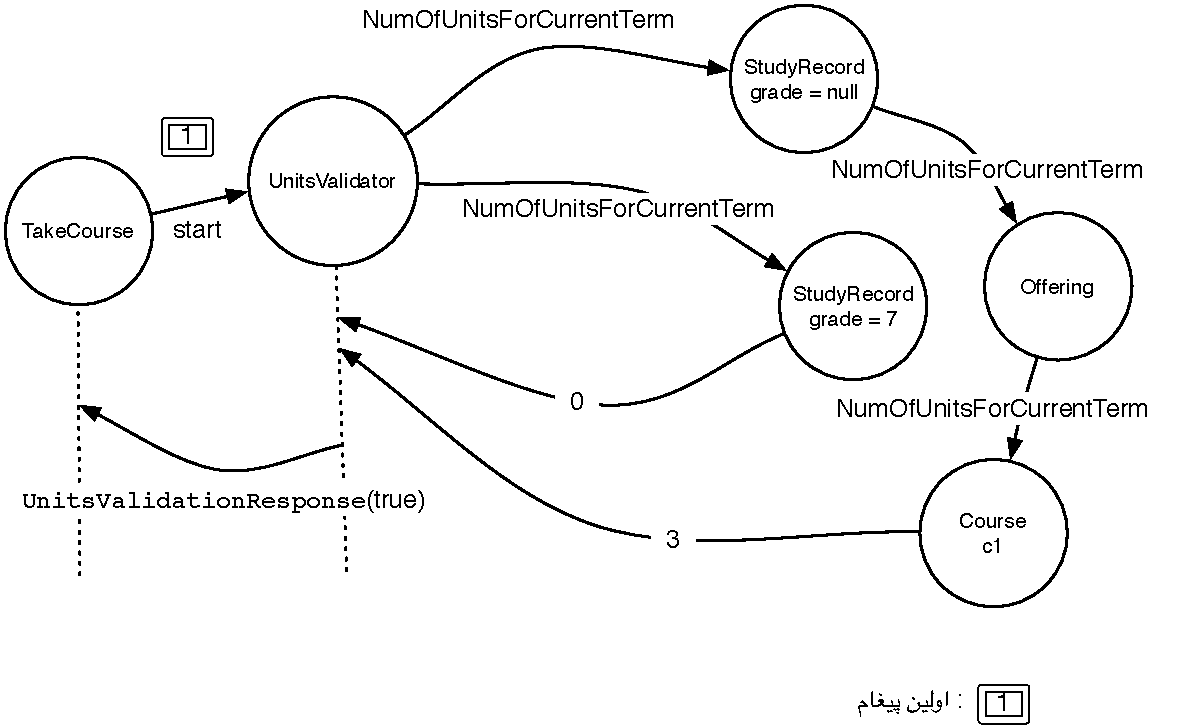
\includegraphics[width=14cm]{4-ProposedFramework/Figures/NumOfUnits.pdf}
    \end{center}
    \caption{\label{fig:take_course_units}نمایش شماتیک تبادل پیغام بین اکتورهای مختلف برای بررسی عدم اخذ بیش از ۲۰ واحد}
\end{figure*}


\section{الگوهای طراحی استخراج شده و نکات مهم}
در این بخش الگوهای طراحی و نکات مهمی‌ که در طول انجام طراحی موارد کاربرد به دست آمده است گردآوری و ارائه شده است. نحوه‌ی تقسیم‌بندی موارد این بخش به این صورت است که ابتدا الگوهای  کلی همکاری اکتورها برای پیاده‌سازی منطق دامنه برشمرده شده‌اند و برای هر مورد سعی شده تأثیر منطق دامنه در انتخاب الگو و نیز در نحوه‌ی پیاده‌سازی جزئیات الگو در نظر گرفته شود. در ادامه الگوها و نکته‌های مهم در طراحی پیغام‌ها ارائه شده‌اند. نهایتا نکات و تجربیاتی که در زمینه‌ی طراحی به روش انتقال ناهمگام و تفاوت‌های مهم آن با طراحی شیءگرای ترتیبی ارائه شده است.
\subsection{الگوهای همکاری اکتورها}
\subsubsection{الگوی انشعاب و الحاق}

\begin{itemize}
\item\textbf{نحوه‌ی پیاده‌سازی به روش تبادل ناهمگام پیغام:}\\
همان‌طور که از نام این الگو بر می‌آید پیاده‌سازی آن از دو بخش تشکیل شده است. برای عمل انشعاب یک اکتور به تعدادی اکتور دیگر که به آنها دسترسی دارد و یا خود آنها را ایجاد می‌کند پیغام‌هایی می‌فرستد. این اکتورها تمام عملیات لازم برای تهیه‌ی پاسخ را انجام داده و پیغام‌های پاسخ را برای اکتور اصلی ارسال می‌کنند. مرحله‌ی جمع‌آوری پیغام‌ها انشعاب نامیده می‌شود. اکتور اصلی این پیغام‌‌ها را دریافت کرده و محاسبات لازم را روی آنها انجام می‌دهد. و در پاسخ عملیات را به صورت پیغام ارسال می‌کند.‍ شکل \ref{fig:fork_and_join} شمایی از این الگو را نشان می‌دهد.
\begin{figure*}
    \begin{center}
	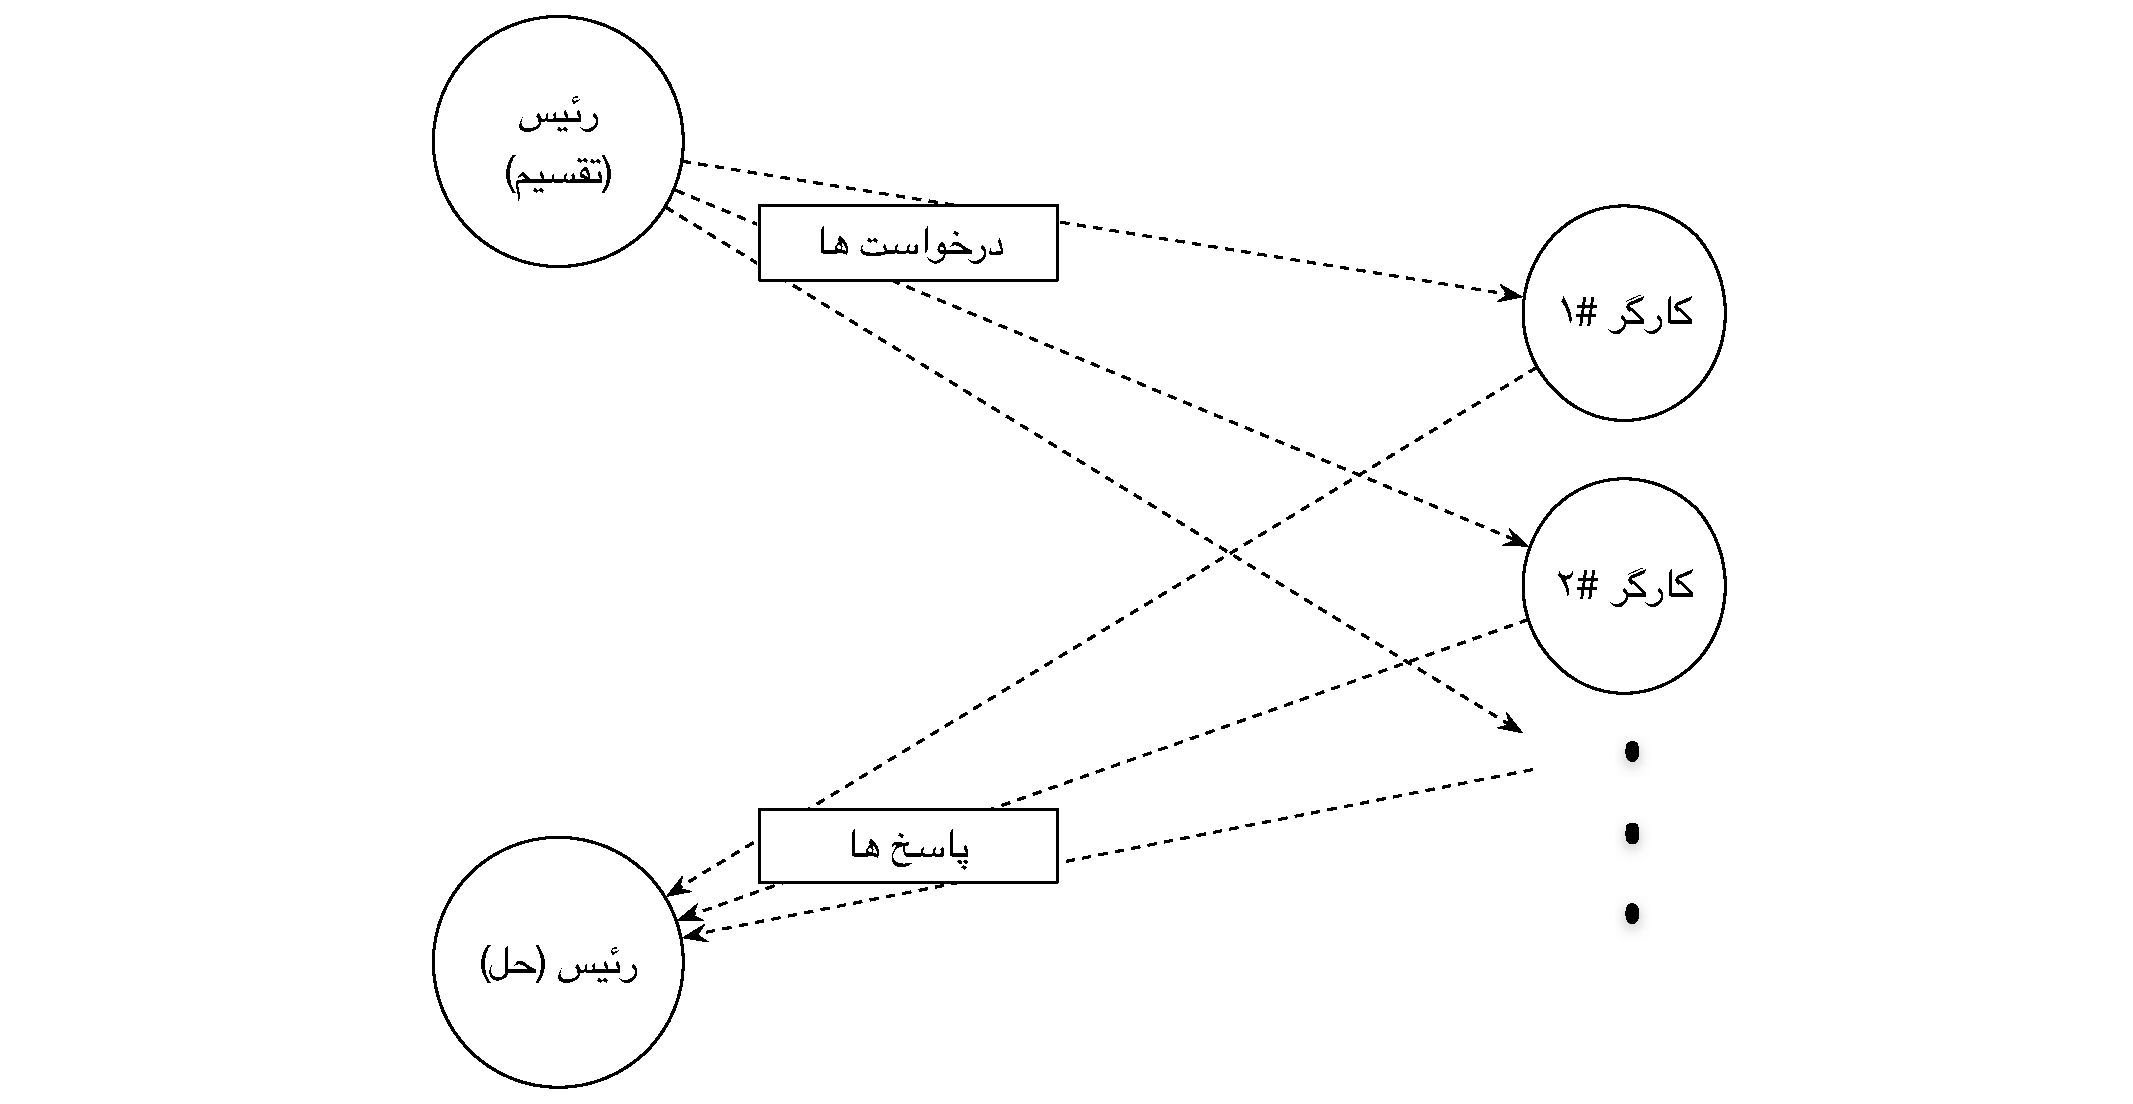
\includegraphics[width=16cm]{3-RelatedWork/Figures/Divide_and_Conquer.pdf}
    \end{center}
    \caption{\label{fig:fork_and_join}  شمای کلی از الگوی انشعاب و الحاق در مدل اکتور }
\end{figure*}

\item\textbf{موارد استفاده}\\
این الگو برای حالاتی از منطق دامنه به کار می‌رود که مسئله از نوع تقسیم و حل است (رجوع کنید به بخش \ref{section:actorPatterns}). مثالی از این کارکرد در مورد کاربرد محاسبه‌ی معدل (جدول \ref{table:uc_gpa}) در بخش قبل مورد بررسی قرار گرفته است. در این مثال، اکتوری که وظیفه‌ی محاسبه‌ی معدل را بر عهده دارد به اکتورهای سابقه‌ی تحصیلی دانشجو دسترسی دارد و برای محاسبه‌ی معدل نیاز به اطلاعاتی دارد که این اکتورها به آن دسترسی دارند. استفاده از الگوی انشعاب و الحاق در این مثال به این صورت است که اکتور محاسبه‌ی معدل پیغام‌های درخواست اطلاعات نمره را برای تمام اکتورهای سابقه ارسال می‌کند (انشعاب)، این اکتورها با برقراری ارتباط با سایر اکتورها موجب می‌شوند اطلاعات لازم به صورت پیغام‌هایی برای اکتور محاسبه‌ی معدل ارسال شود. اکتور محاسبه‌ی معدل با گرفتن پیغام‌ها (الحاق) عملیات مورد نیاز برای محاسبه‌ی معدل را انجام‌ می‌دهد و معدل را به صورت پیغام برای اکتور مقصد ارسال می‌کند.
%موارد استفاده‌ی دیگری هم دارد.؟

\item\textbf{نکات مهم}\\
\begin{enumerate}
\item مناسب بودن مسائل تقسیم و حل برای این الگو به این معنی نیست که نمی‌توان از روش دیگری این مسائل را حل کرد. به عنوان مثال، مورد کاربرد محاسبه‌ی معدل در رویکرد  اول طراحی که در بخش \ref{gpa_approach1} توضیح داده شد، بدون استفاده از این الگو طراحی گردید. همان‌طور که در مقایسه‌ی دو رویکرد مذکور بیان شد، تفاوت استفاده و عدم استفاده از الگوی انشعاب و الحاق صرفا کیفیت طراحی می‌باشد و از نظر صحت عملکرد دو الگو یکسان هستند. بنابراین استفاده از این الگو بیشتر به تمرین در طراحی نیازمند است و صرفاً از روی منطق دامنه قابل تشخیص نیست.
\item مورد دیگر این است که در بسیاری از موارد، استفاده از این الگو به ذهن برنامه‌نویس این طور القا می‌کند که اکتورهایی که انشعاب شده‌اند موظف به فرستادن نتیجه به اکتور اصلی هستند. باید دقت شود که استفاده از این الگو مستقل از این مورد است که نتیجه‌ی کارهای تقسیم شده به چه شکلی به دست اکتور اصلی می‌رسد. همان‌طور که در رویکرد دوم طراحی مورد کاربرد محاسبه‌ی معدل مشاهده شد، پاسخ اکتور محاسبه‌ی معدل می‌تواند از سوی اکتور ترم و یا اکتور درس ارسال شود.
\item استفاده از این الگو صرفا با کشف مورد استفاده به اتمام نمی‌رسد. پس از تصمیم به استفاده از این الگو، تصمیمات دیگری در پاسخ به سؤالاتی از این قبیل باید اتخاذ شود: آیا  اکتور جاری که منطق مطابق با الگو در آن کشف شده است باید به عنوان اکتوری که انشعاب در نظر گرفته شود یا اکتور دیگری به این منظور ایجاد شود؟ آیا اکتور الحاق و اکتور انشعاب یکسان باشند یا اکتور دیگری عمل انشعاب را انجام دهد؟ آیا نتیجه‌ی عملیات حاصل از الگو به اکتور جاری فرستاده شود یا مستقیماً به گیرنده‌ی دیگری ارسال شود؟ 
\end{enumerate} 

\end{itemize}

\subsubsection{الگوی خط لوله}

\begin{itemize}
\item\textbf{نحوه‌ی پیاده‌سازی به روش تبادل ناهمگام پیغام:}\\
پیاده‌سازی این الگو به این صورت است که هر اکتور بخشی از عملیات منطق دامنه‌ را انجام می‌دهد و با ارسال پیغام به اکتور بعدی ادامه‌ی کار را به آن می‌سپارد.
\begin{figure*}
    \begin{center}
	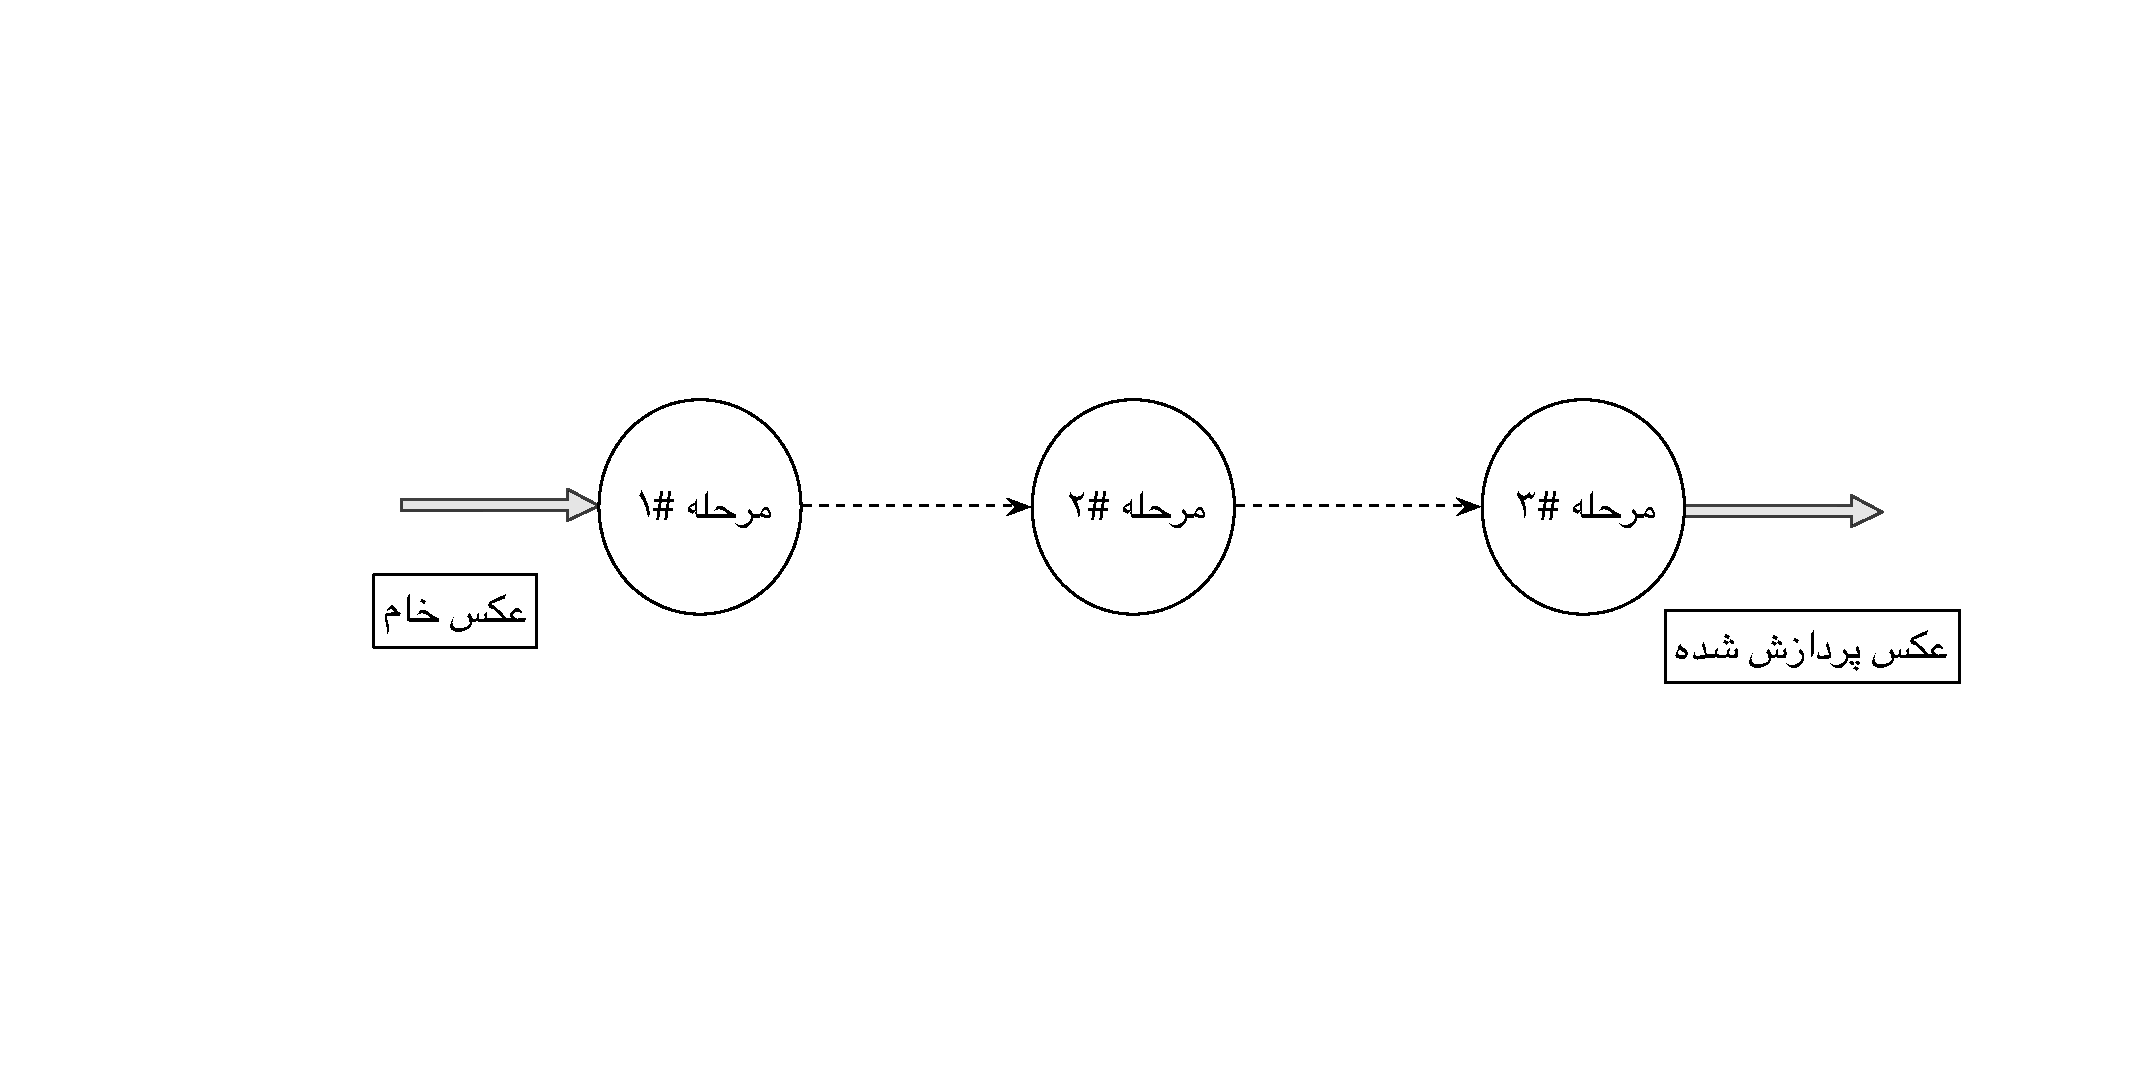
\includegraphics[width=16cm]{3-RelatedWork/Figures/pipeline.pdf}
    \end{center}
    \caption{\label{fig:pipeline_2}  مثالی از الگوی خط لوله }
\end{figure*}

\item\textbf{موارد استفاده}\\
این الگو در دو حالت مورد استفاده قرار می‌گیرد. حالت اول مواردی را شامل می‌شود که خود منطق دامنه نیاز به ترتیب دارد. در این حالت‌ها عملی که در هر مرحله انجام‌ می‌گیرد به صورت منطقی وابسته به نتیجه‌ی مرحله‌ی قبل است. حالت دوم زمانی اتفاق می‌افتد که منطق دامنه نیاز به ترتیب ندارد ولی دسترسی اکتورها به صورت زنجیره‌ای است. مثالی از این حالت،‌ در مورد کاربرد محاسبه‌ی معدل در بخش قبل دیده شد. در این مثال اکتور سابقه، نمره‌ی دانشجو را برای معدل فراهم می‌کند و اکتور درس تعداد واحد‌های درس مربوطه را. با اینکه این دو عمل مستقل از هم بوده و می‌توانند به صورت موازی اجرا شوند،‌ مدل دامنه‌ی سیستم ایجاب می‌کند که پیغام از طریق اکتور سابقه به اکتور ارائه منتقل شود و از طریق این اکتور به دست اکتور درس برسد.

\item\textbf{نکات مهم}\\
\begin{enumerate}
\item مناسب بودن م\textsl{سائل تقسیم و حل} برای این الگو به این معنی نیست که نمی‌توان از روش دیگری این مسائل را حل کرد. به عنوان مثال، مورد کاربرد محاسبه‌ی معدل در رویکرد  اول طراحی که در بخش \ref{gpa_approach1} توضیح داده شد، بدون استفاده از این الگو طراحی گردید. همان‌طور که در مقایسه‌ی دو رویکرد مذکور بیان شد، تفاوت استفاده و عدم استفاده از الگوی انشعاب و الحاق صرفا کیفیت طراحی می‌باشد و از نظر صحت عملکرد دو الگو یکسان هستند. بنابراین استفاده از این الگو بیشتر به تمرین در طراحی نیازمند است و صرفاً از روی منطق دامنه قابل تشخیص نیست.
\item مورد دیگر این است که در بسیاری از موارد، استفاده از این الگو به ذهن برنامه‌نویس این طور القا می‌کند که اکتورهایی که انشعاب شده‌اند موظف به فرستادن نتیجه به اکتور اصلی هستند. باید دقت شود که استفاده از این الگو مستقل از این مورد است که نتیجه‌ی کارهای تقسیم شده به چه شکلی به دست اکتور اصلی می‌رسد. همان‌طور که در رویکرد دوم طراحی مورد کاربرد محاسبه‌ی معدل مشاهده شد، پاسخ اکتور محاسبه‌ی معدل می‌تواند از سوی اکتور ترم و یا اکتور درس ارسال شود.
\item استفاده از این الگو صرفا با کشف مورد استفاده به اتمام نمی‌رسد. پس از تصمیم به استفاده از این الگو، تصمیمات دیگری در پاسخ به سؤالاتی از این قبیل باید اتخاذ شود: آیا  اکتور جاری که منطق مطابق با الگو در آن کشف شده است باید به عنوان اکتوری که انشعاب در نظر گرفته شود یا اکتور دیگری به این منظور ایجاد شود؟ آیا اکتور الحاق و اکتور انشعاب یکسان باشند یا اکتور دیگری عمل انشعاب را انجام دهد؟ آیا نتیجه‌ی عملیات حاصل از الگو به اکتور جاری فرستاده شود یا مستقیماً به گیرنده‌ی دیگری ارسال شود؟ 
\end{enumerate} 

\end{itemize}
